\documentclass[10pt,a4paper]{article}
\usepackage{geometry}
\geometry{a4paper,total={170mm,257mm},left=20mm,top=20mm}
\usepackage[utf8]{inputenc}
\usepackage{amsthm,amssymb,amsmath,natbib,graphicx,caption}
\usepackage{xcolor,enumitem}
\usepackage[ruled,vlined]{algorithm2e}
\setcitestyle{numbers,comma,square}
\usepackage{tikz}
\usetikzlibrary{matrix,calc}
\usepackage{xurl}
\usepackage[pdfpagelabels,hypertexnames=false,bookmarksopen=true,
bookmarksopenlevel=1,colorlinks=true,pdfstartview=FitV,
linkcolor=blue,citecolor=blue,urlcolor=cyan]{hyperref}
\usepackage{cleveref}
\hypersetup{pdftitle={A Deterministic Algorithm for Eigenvalue Separation in Tridiagonal Matrices},pdfauthor={Wenqi Zhu and Ping Nie}}

\newtheorem{proposition}{Proposition}[section]
\newtheorem{theorem}{Theorem}[section]
\newtheorem{corollary}{Corollary}[section]
\newtheorem{lemma}{Lemma}[section]
\newtheorem{example}{Example}[section]
\newtheorem{remark}{Remark}[section]
\newtheorem{assumption}{Assumption}
\newtheorem{definition}{Definition}[section]
\newcommand{\norm}[1]{\left\lVert #1\right\rVert}
\DeclareMathOperator{\gap}{gap}
\DeclareMathOperator{\diag}{diag}
\DeclareMathOperator{\tr}{tr}
\DeclareMathOperator{\rank}{rank}
\DeclareMathOperator{\spn}{span}
\newcommand{\R}{\mathbb R}
\newcommand{\C}{\mathbb C}
\renewcommand{\baselinestretch}{1.25}
\title{A Deterministic Algorithm for Eigenvalue Separation\\in Tridiagonal Matrices}
\author{%
Wenqi Zhu\thanks{Corresponding author.}\\
{\small Mathematical Institute, Woodstock Road, University of Oxford,}\\
{\small Oxford, UK, OX2 6GG}\\
{\small\texttt{wenqi.zhu@maths.ox.ac.uk}}\\[1ex]
Ping Nie\\
{\small David R. Cheriton School of Computer Science, University of Waterloo}\\
{\small\texttt{ping.nie@uwaterloo.ca}}}
\date{}
\begin{document}
\maketitle

\begin{abstract}
We develop a deterministic algorithm for separating the eigenvalues
of Hermitian tridiagonal matrices by small diagonal perturbations.
For $\|T\|_2\leq1$, $0<\delta<1/2$, and
$X=\diag(1,\ldots,n)$, our algorithm selects $t\in[0,\delta/n]$ such
that $D=tX$ satisfies
\[
\|D\|_2\leq\delta,
\qquad
\gap(T+D)>2^{-34}\delta^2n^{-12}.
\]
The construction uses a classical convex weighted eigenvalue sum and its
finite-scale slope variation. A tridiagonal localization argument turns
near-degenerate eigenvalues into separated responses to the fixed diagonal
direction, yielding a quantitative gap certificate. An adaptive interval
selector then identifies a certifying window in at most
$\lceil\log_2(16n^3)\rceil$ refinements. With the exact-arithmetic
spectral-function oracle constructed in the appendix, the algorithm
uses $O(n[1+\log(n/\delta)]^3)$ arithmetic operations, comparisons
and square roots in total, a nearly linear exact-arithmetic
complexity bound. As a numerical illustration, a structure-exploiting
implementation uses rigorous
Sturm eigenvalue enclosures and adaptive precision to certify the
stopping condition on six families of test matrices. The directly
certified gaps are substantially larger than the worst-case analytical
bounds, illustrating both the effectiveness of the construction and the
conservatism of the universal certificate. Our results address the
nearly linear deterministic Minami perturbation question for
tridiagonal matrices.
\end{abstract}


\section{Introduction}
\label{sec:problem}

Spectral separation plays an important role in numerical linear
algebra. When eigenvalues are tightly clustered, computing their
individual eigenvectors and associated invariant subspaces can
become sensitive to perturbations. Spectral gaps also influence
the accuracy, convergence, and deflation criteria of many
eigenvalue algorithms \cite{Parlett1996,Nakatsukasa2012,
HorningTownsend2020}. A natural approach is to perturb the
matrix slightly so that its eigenvalues become better separated.
The challenge is to construct such a perturbation efficiently,
without first computing an expensive eigendecomposition.

Diagonal perturbations are particularly attractive for
tridiagonal matrices because they preserve the matrix structure
and the cost of matrix-vector products. In random spectral
theory, Minami-type estimates provide probabilistic bounds on
the occurrence of closely clustered eigenvalues under suitable
independent diagonal perturbations
\cite{Minami1996,CombesGerminetKlein2009}. Whether comparable
separation can be achieved deterministically is a more
challenging question. It was posed as Problem~3.2,
\emph{Deterministic Minami Perturbation}, in the report of the
Simons Institute workshop \emph{Linear Systems and Eigenvalue
Problems}, held in Berkeley in October 2025
\cite{AmselEtAl2026}. The KE-02 entry in the Open Problems
in NLA catalogue further asks for a nearly linear deterministic
construction for arbitrary normalized Hermitian tridiagonal
matrices \cite{CatalogueKE02}.

Let $n\geq2$, $0<\delta<1/2$, and let $T\in\C^{n\times n}$
be Hermitian tridiagonal with $\norm{T}_2\leq1$. Thus
\begin{equation}\label{eq:T}
T=\begin{pmatrix}
d_1&\beta_1&&&\\
\overline{\beta_1}&d_2&\beta_2&&\\
&\overline{\beta_2}&d_3&\ddots&\\
&&\ddots&\ddots&\beta_{n-1}\\
&&&\overline{\beta_{n-1}}&d_n
\end{pmatrix},\qquad d_i\in\R.
\end{equation}
We write its eigenvalues in nondecreasing order and
define its minimum eigenvalue gap by
\begin{equation}\label{eq:gap}
\gap(T):=\min_{1\leq j<n}
\bigl(\lambda_{j+1}(T)-\lambda_j(T)\bigr).
\end{equation}
In particular, $\gap(T)=0$ if $T$ has a repeated eigenvalue.
The objective is to construct a real diagonal matrix $D$
such that
\begin{equation}\label{eq:target}
\norm{D}_2\leq\delta,\qquad
\gap(T+D)\geq c_0(\delta/n)^a,
\end{equation}
for absolute constants $c_0,a>0$, at a total cost of
$O\bigl(n[1+\log(n/\delta)]^q\bigr)$ exact arithmetic
operations for a constant $q$.
This cost concerns the construction of $D$, including
any internal spectral evaluations; it does not require
outputting an eigenvector matrix. Arithmetic complexity
and finite-precision complexity are separate questions.

Several related approaches provide insight into this problem.
Classical work by Ye~\cite{Ye1995} and
Parlett~\cite{Parlett1996} explains how closely spaced
eigenvalues of tridiagonal matrices are associated with
the localization of their invariant subspaces.
Nakatsukasa~\cite{Nakatsukasa2012} uses bounds on
eigenvector components to study the sensitivity of
eigenvalues to structured perturbations.
More recently, deterministic constructions have been
obtained for special classes, including weakly coupled
tridiagonal matrices and matrices with constant diagonal
and equal off-diagonal magnitudes
\cite{CatalogueKE02}. These results provide important
structural insights, but do not establish the requested
nearly linear construction for the unrestricted
tridiagonal case.

In this paper, we give a deterministic construction for
the full Hermitian tridiagonal class. Our approach takes
a different perspective: rather than estimating individual
eigenvalue movements directly, we use the convexity of a
weighted spectral function to detect and avoid regions of
strong spectral sensitivity.
In particular, we restrict the perturbation to a
single predetermined diagonal direction:
\begin{equation}\label{eq:tilt}
\boxed{
X=\diag(1,\ldots,n),\qquad
H(t)=T+tX,\qquad 0\leq t\leq\delta/n.
}
\end{equation}
Since $\norm{tX}_2=nt\leq\delta$, every parameter in this
interval respects the perturbation budget. The matrix
search therefore reduces to selecting one scalar $t$.
The remaining issue is to certify spectral separation at
the selected parameter without first computing the
minimum gap accurately.

Our main result is the following theorem. It combines
\Cref{thm:selection} with \Cref{lem:oracle}; the proof is
completed in \Cref{subsec:oracle}.

\begin{theorem}[Main theorem]\label{thm:main}
Let $n\geq2$, $0<\delta<1/2$, and let $T\in\C^{n\times n}$ be
Hermitian tridiagonal with $\norm{T}_2\leq1$.
The deterministic \Cref{alg:selection}, with the
spectral-function oracle of \Cref{lem:oracle}, computes
$t\in[0,\delta/n]$ and outputs the real diagonal matrix $D=tX$,
using $n$ further multiplications; this matrix satisfies
\begin{equation}\label{eq:main}
\boxed{
\norm{D}_2\leq\delta,
\qquad
\gap(T+D)>2^{-34}\frac{\delta^2}{n^{12}}
\geq2^{-34}\Bigl(\frac{\delta}{n}\Bigr)^{12}.
}
\end{equation}
It uses $O\bigl(n[1+\log(n/\delta)]^3\bigr)$ arithmetic
operations, comparisons and square roots in total.
The model of computation is exact real arithmetic and
comparisons, with unit-cost square roots of nonnegative real
numbers and complex numbers represented as pairs of real
numbers; no logarithm, floor or bit extraction is used as a
primitive operation, and the integers needed by the algorithm
are computed by doubling and comparisons, at counted cost. Thus \eqref{eq:target} holds with $c_0=2^{-34}$,
$a=12$ and $q=3$.
\end{theorem}

\paragraph{Main results and contributions.}
This paper delivers two main results.

\emph{First, we develop a convex spectral-gap certificate.}
We consider a weighted sum of the ordered eigenvalues
of $H(t)$, viewed as a function $F(t)$ of the perturbation
parameter. This spectral function is convex, strictly
increasing, and has bounded slopes with respect to the perturbation size $t$. Up to an affine
trace term, it measures the total pairwise spectral
distance after perturbation. By the Hellmann--Feynman formula, its first
derivative is a weighted sum of the responses of
individual eigenvalues to the diagonal perturbation.
Moreover, classical second-order perturbation formulas
show that the curvature contains pairwise contributions
of the form
\[
\underbrace{\text{curvature contribution}}_{
\text{for a pair of eigenvalues}}
\ \propto\
\frac{|\text{perturbation coupling}|^2}
{\text{eigenvalue gap}}.
\]
Thus closely spaced eigenvalues can produce a strong
change in spectral slope, provided that their responses
to the perturbation are sufficiently different.

The difficulty is that a small gap alone does not
guarantee large curvature: the corresponding coupling
may be weak or vanish. To overcome this, we exploit
the tridiagonal structure. A discrete Wronskian
identity and a small-leakage cut convert a nearly
degenerate eigenvalue pair into two spatially
separated approximate eigenvectors. Their responses
to the fixed diagonal direction $X$ are quantitatively
different. Using a nearby auxiliary matrix and the
variational representation of the spectral function,
we turn this response separation into a finite-scale
gap certificate.

This proof combines ideas from classical eigenvector
localization and structured perturbation theory
\cite{Ye1995,Parlett1996,Nakatsukasa2012}
with convex spectral analysis
\cite{OvertonWomersley1993,Lewis1996Convex,
LewisSendov2001}. The key is to use these classical
tools for a different purpose: instead of bounding
the sensitivity of a given eigenvalue or optimizing
a spectral objective, we certify a lower bound on
the minimum spectral gap.

\emph{Second, we construct an adaptive deterministic
interval-selection algorithm.}
Starting from the admissible parameter interval
$[0,\delta/n]$, the algorithm repeatedly selects
one of two shorter windows, each retaining slightly
less than half of the current interval. Convexity
allows us to compare their endpoint slope variations
and choose a window with a smaller spectral response.
At every iteration, we directly test whether the
centered slope variation is sufficiently small to
certify spectral separation. Once this condition
is satisfied, the algorithm terminates. 

Each refinement requires only a constant number
of evaluations of the spectral function. In
particular, the selection rule does not require
prior knowledge of the eigenvectors or a full
eigendecomposition at each step. We prove that
the algorithm terminates after at most
\[
K=\left\lceil\log_2(16n^3)\right\rceil
=O(\log n)
\]
refinements. The returned perturbation satisfies
\begin{equation}\label{eq:intro-main-result}
\boxed{
\norm{tX}_2\leq\delta,\qquad
\gap(T+tX)>2^{-34}\,\frac{\delta^2}{n^{12}}.
}
\end{equation}
Including the cost of the spectral-function oracle of
\Cref{app:oracle}, the construction requires
$O(n[1+\log(n/\delta)]^3)$ arithmetic operations,
comparisons and square roots; see \Cref{thm:main}.
Thus the algorithm meets the nearly linear
arithmetic-complexity target of KE-02 for
general Hermitian tridiagonal matrices. 
The two contributions are complementary:
the first provides a local certificate relating
spectral response to eigenvalue separation, while
the second uses convexity to find a certifying
perturbation parameter efficiently.

\paragraph{Numerical illustration.}
We implement the adaptive algorithm using
double-precision window selection, rigorous
Sturm-based eigenvalue enclosures, and adaptive
precision. Experiments on six families of
tridiagonal matrices show that the certified
stopping condition is often satisfied well
before the theoretical iteration bound.
The reported instances have orders up to $n=500$
(Section~\ref{sec:numerics}). Directly certified
eigenvalue gaps are many orders of magnitude
larger than the analytical lower bounds. These
results demonstrate the practical effectiveness
of the construction on the tested instances,
without implying an improved worst-case exponent.

\paragraph{Related work: localization and structured perturbation.}
Classical work on close eigenvalues of tridiagonal
matrices provides an important foundation for our
geometric argument. Ye~\cite{Ye1995} relates
closely spaced eigenvalues to complementary
principal submatrices, even when the off-diagonal
entry connecting the two blocks is not small.
Parlett~\cite{Parlett1996} studies the localization
of invariant subspaces associated with tightly
clustered eigenvalues, while V{\"o}mel and
Parlett~\cite{VoemelParlett2011} investigate
how such localization can be detected.

These results show that small spectral gaps
are closely connected to the spatial structure
of the corresponding eigenspaces. Our localization
argument follows this viewpoint, but requires a
specific quantitative conclusion: two approximate
eigenvectors supported on opposite sides of
a coordinate cut, with small residuals and
separated responses to the predetermined
direction $X$. 
Nakatsukasa~\cite{Nakatsukasa2012} develops
a complementary perturbation approach for
Hermitian block tridiagonal matrices. By
bounding eigenvector components through the
block recurrence, he obtains upper bounds
on the movement of individual eigenvalues
under structured perturbations, with applications
to Wilkinson matrices and aggressive early
deflation. In contrast, we use the localization
of a near-degenerate pair to establish a lower
bound on its collective spectral response.
This response is then converted into a
minimum-gap certificate through convexity.
Thus our work connects the geometric ideas
of tridiagonal localization to a different
spectral-certification problem.

\paragraph{Related work: convex eigenvalue optimization.}
Weighted eigenvalue sums and diagonal matrix
corrections have a long history in spectral
optimization, including graph partitioning
and nondifferentiable optimization
\cite{DonathHoffman1973,CullumDonathWolfe1975,
LewisOverton1996}.
Ky Fan's variational principle and subsequent
work of Overton and Womersley, Lewis, and
Lewis--Sendov establish the convexity,
subdifferential, and second-order calculus
of spectral functions
\cite{Fan1949,OvertonWomersley1992,
OvertonWomersley1993,Lewis1996Convex,
Lewis1996Derivatives,LewisSendov2001}. 
These classical results are key to our spectral function. In eigenvalue
optimization, such functions have typically
been used to characterize optimality, derive
subgradients, or construct optimization
algorithms. Here we use the same variational
structure in a different direction. 
In particular, our proof uses the existence
of distinct supporting spectral slopes at
a nearby matrix with a repeated eigenvalue.
The difference between these slopes is
controlled by the responses of two localized
eigenvectors to $X$. We then transfer this
information back to the original matrix
using stability of the convex spectral
function. This is the central connection
between structured eigenvalue perturbation
and nonsmooth convex analysis in our proof. 

Rather than minimizing the spectral function,
we search for a window on which its finite-scale
slope variation is small. Such a window certifies
that the spectrum is sufficiently separated.
The interval-selection mechanism is also related
to adaptive sampling of convex functions.
Simchowitz et al.~\cite{SimchowitzEtAl2018},
for example, use midpoint secant errors to
guide the approximation of a convex function.
Their midpoint error is directly related to
our centered slope variation.

\paragraph{Notation.}
We use $\norm{\cdot}_2$ for the Euclidean vector norm
and the matrix operator norm, $\norm{\cdot}_{\mathrm F}$
for the Frobenius norm, and $\norm{\cdot}_*$ for the
nuclear norm, the sum of the singular values.
The vector $e_i$ is the $i$th standard unit vector.
At every permitted parameter,
$\norm{H(t)}_2\leq1+\delta<2$, and its off-diagonal
entries have absolute value at most one.

\begin{remark}[Reduction to real symmetric matrices]
\label{rem:real}
A diagonal unitary matrix $S$ can be chosen so that
$S^*TS$ is real symmetric. Choose its phases
successively along each chain of nonzero
off-diagonal entries; zero entries separate
the chains. Since $S^*XS=X$, the entire family
$T+tX$ is preserved up to unitary similarity.
Thus the eigenvalues, gaps, and norms are
unchanged, and the real symmetric arguments
below also apply to Hermitian tridiagonal matrices.
\end{remark}

The remainder of the paper is organized as follows.
Section~\ref{sec:convex-spectral} develops the
convex spectral function and its finite-scale
slope variation. Section~\ref{sec:local-gap}
uses tridiagonal localization to establish
the local gap certificate.
Section~\ref{sec:selection} develops a basic
and an improved adaptive window selector
and analyzes spectral-function evaluations.
Section~\ref{sec:numerics} presents numerical
illustrations, in which the stopping test is
rigorously certified along a double-precision
selection path.
Section~\ref{sec:conclusion} summarizes
the results and discusses possible extensions.
\section{The convex spectral function and its slope variation}
\label{sec:convex-spectral}

Throughout this section, the results apply to any Hermitian matrix, not only to tridiagonal matrices. We use the notation $T$ for simplicity. 

\paragraph{The spectral function.}
For the fixed family $H(t)=T+tX$, define the spectral function
\begin{equation}\label{eq:F}
\boxed{F(t):=\sum_{j=1}^n j\lambda_j(H(t)).}
\end{equation}
The map $A\mapsto\sum_{j=1}^n j\lambda_j(A)$ is a convex
spectral function, meaning that it is convex in a Hermitian
matrix $A$ and depends only on its eigenvalues.
Its basic properties follow from Ky Fan's maximum principle
\cite{Fan1949}, which provides a variational characterization
of sums of the largest eigenvalues. Overton and Womersley
\cite{OvertonWomersley1992} further studied these eigenvalue
sums and their convex-analytic properties, while Lewis
\cite{Lewis1996Convex} developed a general convex-analytic
framework for spectral functions on Hermitian matrices.


These variational characterizations have played an
important role in eigenvalue optimization. In particular,
Overton and Womersley~\cite{OvertonWomersley1993}
developed optimality conditions and duality theory
for minimizing sums of the largest eigenvalues.
Closely related weighted trace objectives also appear
in Brockett's work on matrix gradient flows,
eigenvalue ordering, and diagonalization
\cite{Brockett1991}. The weights $1,\ldots,n$
in our spectral function correspond to such a
weighted trace objective through \eqref{eq:variational}.



While these spectral functions and their convexity
properties are classical, our interest is different:
we study their variation along a fixed diagonal
perturbation and use this variation to certify
quantitative eigenvalue separation.


\paragraph{Why this spectral function?}
A useful interpretation follows by collecting coefficients:
\begin{equation}\label{eq:pairwise-spread}
\boxed{F(t)=\frac{n+1}{2}\tr H(t)
+\frac12\sum_{i<j}\bigl(\lambda_j(t)-\lambda_i(t)\bigr).}
\end{equation}
Thus $F$ measures the total pairwise spectral distance,
up to an affine trace term. \Cref{ex:tails} illustrates its
decomposition into sums of the largest eigenvalues and shows
why we instead use its change under perturbation to control
the smallest gap.

\begin{example}[Tail sums and spectral spread]\label{ex:tails}
When $n=3$, the tail-sum decomposition in \eqref{eq:variational} is
\[
F(t)=\lambda_1(t)+2\lambda_2(t)+3\lambda_3(t)
=\underbrace{\lambda_1(t)+\lambda_2(t)+\lambda_3(t)}_{\tr H(t)}
+\underbrace{\lambda_2(t)+\lambda_3(t)}_{\text{two largest}}
+\underbrace{\lambda_3(t)}_{\text{largest}}.
\]
The significance of $F$ lies in its variation under the perturbation $tX$.
As $t$ varies, the eigenvalues move at different rates,
and their pairwise gaps change accordingly. When two
eigenvalues approach one another, their relative motion
may change rapidly, producing curvature in $F$.
This motivates studying the second difference of $F$,
which removes the affine trace contribution and measures
the variation of the spectral spread over a finite
perturbation window. We will use this variation to
derive a certificate for the minimum eigenvalue gap.
\end{example}

The following lemma collects the technical properties of the spectral function needed for our analysis. Note that the variational principle and convexity in \Cref{lem:convex} are classical
\cite{Fan1949,OvertonWomersley1992,Lewis1996Convex}. We give the proof for completeness. 

\begin{lemma}[Properties of the spectral function]\label{lem:convex}
For every Hermitian $T$, the function $F$ is
\textbf{strictly increasing} and \textbf{convex}.
For $u<v$, its secant slopes satisfy
\begin{equation}\label{eq:slopes}
\boxed{
\frac{n(n+1)}2
\leq\frac{F(v)-F(u)}{v-u}
\leq\frac{n^2(n+1)}2.
}
\end{equation}
Moreover, it admits the variational representation
\begin{equation}\label{eq:variational}
F(t)
=\max_{U^*U=I}\tr\bigl(UXU^*(T+tX)\bigr)
=\tr(T+tX)+\sum_{j=2}^n\sum_{\ell=j}^n\lambda_\ell(t).
\end{equation}
\end{lemma}

\begin{proof}
Write $\lambda_\ell(t)=\lambda_\ell(T+tX)$. Counting the
coefficient of each eigenvalue gives
$
F(t)=\tr(T+tX)+\sum_{j=2}^n\sum_{\ell=j}^n\lambda_\ell(t).
$
Ky Fan's maximum principle \cite{Fan1949} states that
\[
\sum_{\ell=n-k+1}^n\lambda_\ell(t)
=\max_{\substack{V\in\C^{n\times k}\\V^*V=I_k}}
\tr\bigl(V^*(T+tX)V\bigr).
\]
For fixed $V$, the expression on the right is affine in $t$.
Its pointwise maximum is therefore convex, and \eqref{eq:variational}
proves the convexity of $F$. To obtain the first equality
in \eqref{eq:variational}, expand the weighted trace in the
same way into a trace term and tail sums of Rayleigh quotients.
Each tail sum is bounded by the corresponding eigenvalue sum,
and all bounds are attained simultaneously in an ordered
orthonormal eigenbasis. When $T$ is real symmetric, the
maximizing matrix may be chosen real orthogonal. 
Finally, since $I\preceq X\preceq nI$, each ordered eigenvalue
increases by an amount between $v-u$ and $n(v-u)$ for $u<v$.
Thus $F$ is strictly increasing with bounded secant slopes.
\end{proof}


\paragraph{Spectral sensitivity under perturbation.}

The connection between the spectral function and
eigenvalue separation can also be understood through
classical perturbation theory. Suppose that $H(t)$
has simple eigenvalues, with normalized eigenvectors
$u_j(t)$. The Hellmann--Feynman formula gives
\begin{equation}\label{eq:spectral-first-derivative}
\lambda_j'(t)=u_j(t)^*Xu_j(t),\qquad
F'(t)=\sum_{j=1}^n j\,u_j(t)^*Xu_j(t).
\end{equation}
Thus the derivative of $F$ is a weighted sum of the
responses of individual eigenvalues to the diagonal
perturbation. Differentiating again and pairing the
eigenvalue terms yields
\begin{equation}\label{eq:spectral-second-derivative}
\boxed{
F''(t)=2\sum_{j<k}
\frac{(k-j)|u_j(t)^*Xu_k(t)|^2}
{\lambda_k(t)-\lambda_j(t)}.
}
\end{equation}
Schematically, each nonzero pairwise contribution obeys
\[
\underbrace{\text{curvature contribution}}_{\text{for a pair of eigenvalues}}
\ \propto\
\frac{|\text{perturbation coupling}|^2}{\text{eigenvalue gap}},
\]
with the precise weight $2(k-j)$ in \eqref{eq:spectral-second-derivative}.
The numerator measures the coupling between the two
eigenvectors induced by $X$, while the denominator
is their eigenvalue separation. Thus small gaps can
produce large curvature when the corresponding
perturbation coupling is non-negligible. Conversely,
a small gap need not produce large curvature if this
coupling is weak. These observations are related to
the differential theory of spectral functions
\cite{Lewis1996Derivatives,LewisSendov2001,
DrusvyatskiyPaquette2018}.



This motivates a finite-scale measure of spectral
sensitivity that remains meaningful when eigenvalues
are repeated and classical derivatives are unavailable.


\paragraph{Computing and interpreting slope variation.}
\begin{definition}[Centered slope variation]\label{def:defect}
For $h>0$, define the centered slope variation of $F$ at $t$ by
\begin{equation}\label{eq:defect}
\boxed{
\mathcal S_h(t)
:=
\frac{F(t+h)-F(t)}h
-
\frac{F(t)-F(t-h)}h
\geq0.
}
\end{equation}
\end{definition}
The quantity $\mathcal S_h(t)$ requires three
spectral-function evaluations and measures the difference
between the right and left secant slopes over the window
$[t-h,t+h]$.  


Equivalently, the slope variation can be written
directly in terms of the ordered eigenvalues:
\begin{equation}\label{eq:slope-eigenvalues}
\boxed{
\mathcal S_h(t)=\sum_{j=1}^n j
\left(
\frac{\lambda_j(t+h)-\lambda_j(t)}{h}
-\frac{\lambda_j(t)-\lambda_j(t-h)}{h}
\right).
}
\end{equation}
Hence $\mathcal S_h(t)$ measures the change in the
weighted average eigenvalue slopes between the
left and right halves of the window. When the
eigenvalues respond approximately linearly to the
perturbation, this variation is small. Rapid changes
in their relative motion, including changes in the
ordering of continuously tracked eigenvalue branches,
can instead produce a large slope variation.

If $F$ is twice continuously differentiable on the window,
the slope variation can also be expressed as
\begin{equation}\label{eq:slope-curvature}
\boxed{
\mathcal S_h(t)
=
\int_{-h}^{h}
\left(1-\frac{|s|}{h}\right)F''(t+s)\,ds.
}
\end{equation}
Thus $\mathcal S_h(t)$ is a weighted
integral of the curvature over the prescribed window.


The perturbation scale offers another interpretation.
If the family is extended to large positive $t$, the
term $tX$ dominates the fixed matrix $T$, and the
eigenvalues satisfy $\lambda_j(t)=jt+O(1)$.
In fact, $F$ becomes asymptotically affine, so
$\mathcal S_h(t)\to0$ for each fixed $h>0$ as
$t\to+\infty$. This is a useful limiting picture,
but it lies outside the small-perturbation regime
required by our problem.



Here $0\leq t\leq\delta/n$, so domination by
$tX$ cannot be assumed. Instead, the convexity
and bounded total slope variation of $F$ allow us
to search for a window with sufficiently stable
spectral response. The local certificate in
\Cref{prop:bridge} shows that, for our normalized
tridiagonal family,
\[
\mathcal S_h(t)<\frac12
\quad\Longrightarrow\quad
\gap(H(t))>\frac{h^2}{2^{20}n^4}.
\]
Thus small slope variation certifies quantitative
separation at the window center. The procedure
in \Cref{sec:selection} then finds such a window.



\begin{example}[A collision produces a corner]
\label{ex:collision}
Let $T=\diag(0.1,0)$ and $X=\diag(1,2)$.
Then $H(t)=\diag(0.1+t,2t)$, whose eigenvalues coincide
at $t=0.1$. Ordering them gives
\begin{equation}\label{eq:collision}
F(t)=
\begin{cases}
0.2+4t,&t\leq0.1,\\
0.1+5t,&t\geq0.1,
\end{cases}
\qquad
F(t)=0.15+4.5t+\frac12|t-0.1|.
\end{equation}
The slope increases from $4$ to $5$. Dividing the centered
second difference by $h$ gives the centered slope variation
\begin{equation}\label{eq:collision-defect-explicit}
\boxed{
\mathcal S_h(t)
=
\frac1{2h}\bigl(
|t+h-0.1|+|t-h-0.1|-2|t-0.1|
\bigr)
=
\max\left\{1-\frac{|t-0.1|}{h},0\right\}.
}
\end{equation}
Thus $\mathcal S_h$ is a triangular peak centered at $t=0.1$; see \Cref{fig:convexity-defect}. 
Since affine terms cancel in the slope difference, the trace
contribution in \eqref{eq:pairwise-spread} does not affect
$\mathcal S_h(t)$. 
\end{example}

\begin{figure}[h]
\centering
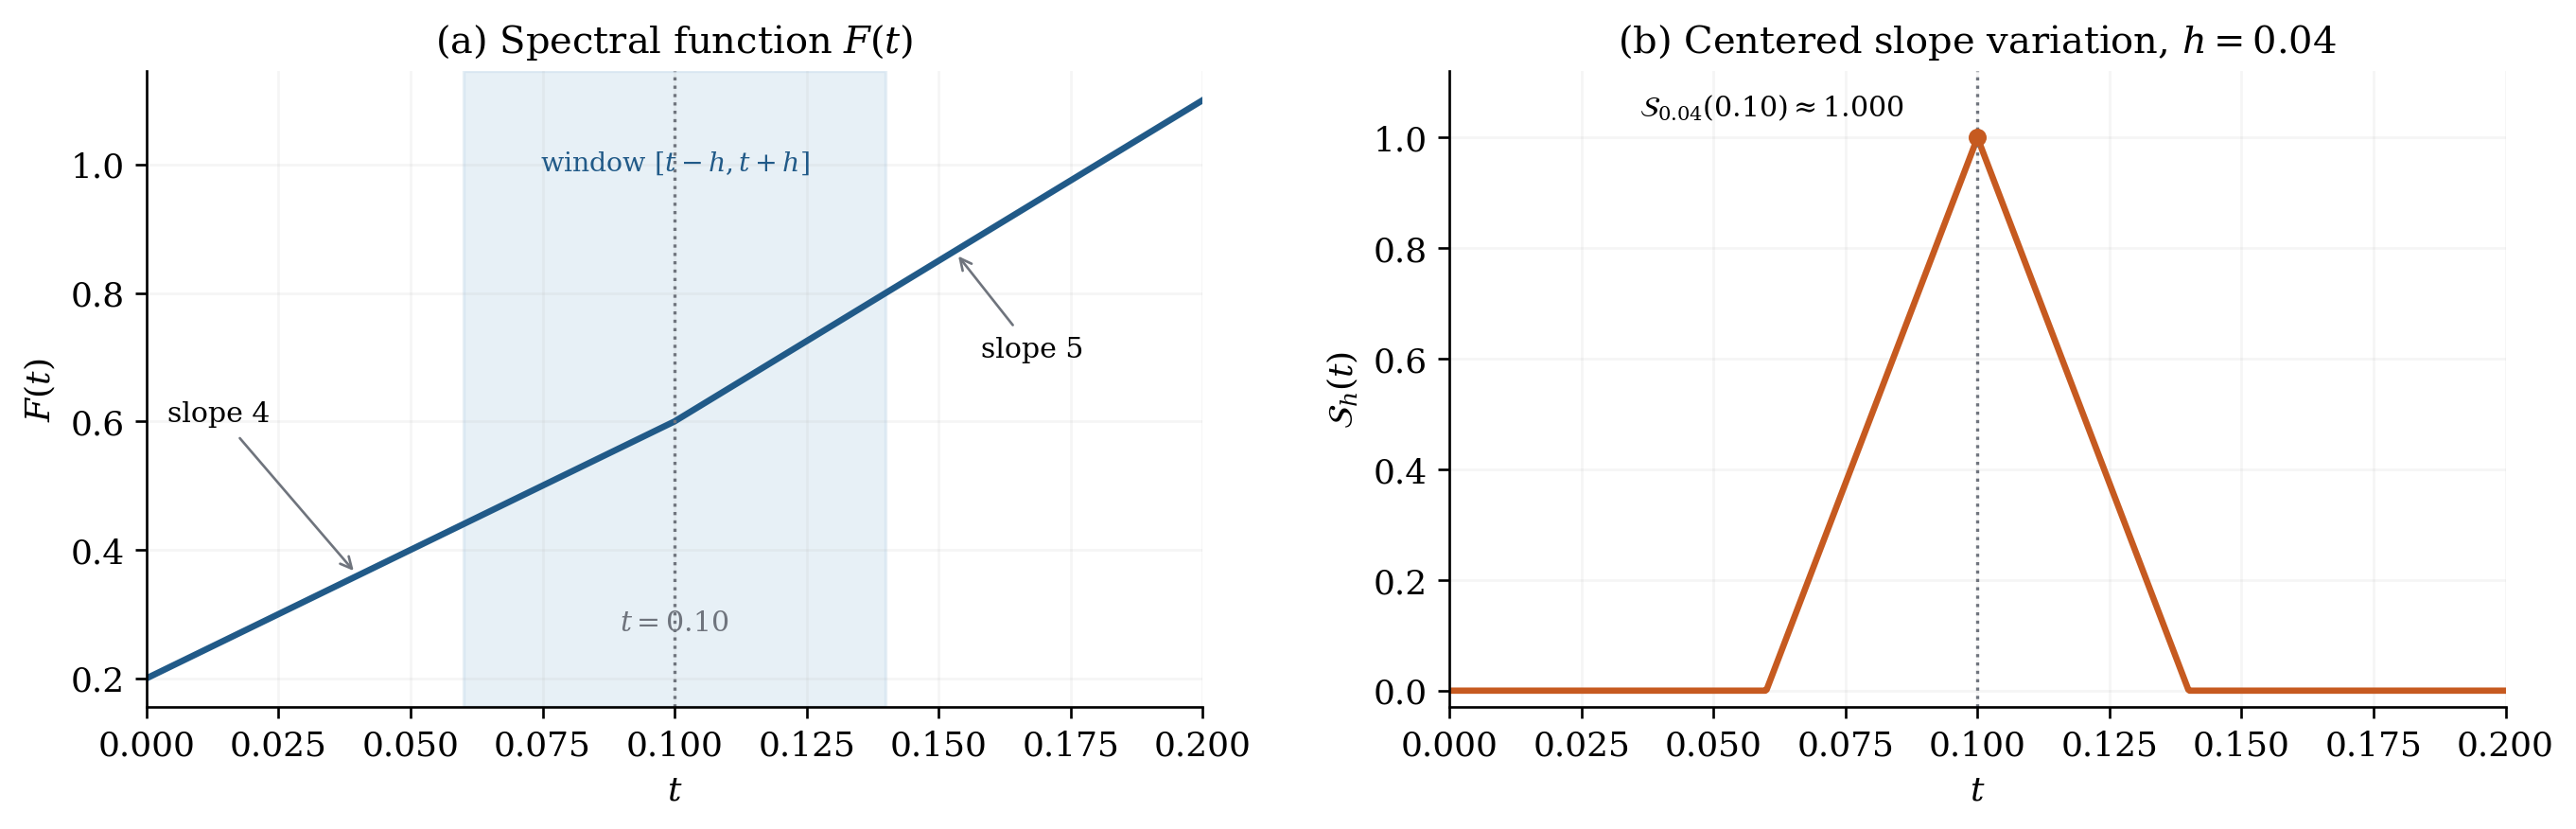
\includegraphics[width=0.98\linewidth]{ke02_collision_slope_variation_updated.png}
\caption{\Cref{ex:collision} with $h=0.04$.
Left: the spectral function $F(t)$, with the window
$[t-h,t+h]$ highlighted around $t=0.1$.
The slope increases from $4$ to $5$ at the center.
Right: the corresponding centered slope variation
$\mathcal S_h(t)$, which forms a triangular peak
of height $1$ at $t=0.1$.}
\label{fig:convexity-defect}
\end{figure}

\begin{example}[A tridiagonal matrix with avoided crossings]
\label{ex:tridiagonal-defect}
Let
\begin{equation}\label{eq:tridiagonal-example}
T=
\begin{pmatrix}
0.16&0.003&0\\
0.003&0.10&0.003\\
0&0.003&0
\end{pmatrix},
\qquad
X=\diag(1,2,3).
\end{equation}
Both off-diagonal edges are nonzero, so $T+tX$ has
simple eigenvalues for every $t$. Thus $F$ and $\mathcal S_h(t)$ are smooth.
\Cref{fig:tridiagonal-defect} shows the local bend and
the slope variation over a larger range of centers.
There are three visible peaks near $0.06,0.08,0.10$,
the crossing locations of the diagonal branches when
the edges are set to zero. With the nonzero edges in
\eqref{eq:tridiagonal-example}, these are smooth peaks,
not exact corners. These computations illustrate the
slope variation; they are not certified numerical bounds.
\end{example}

\begin{figure}[h]
\centering
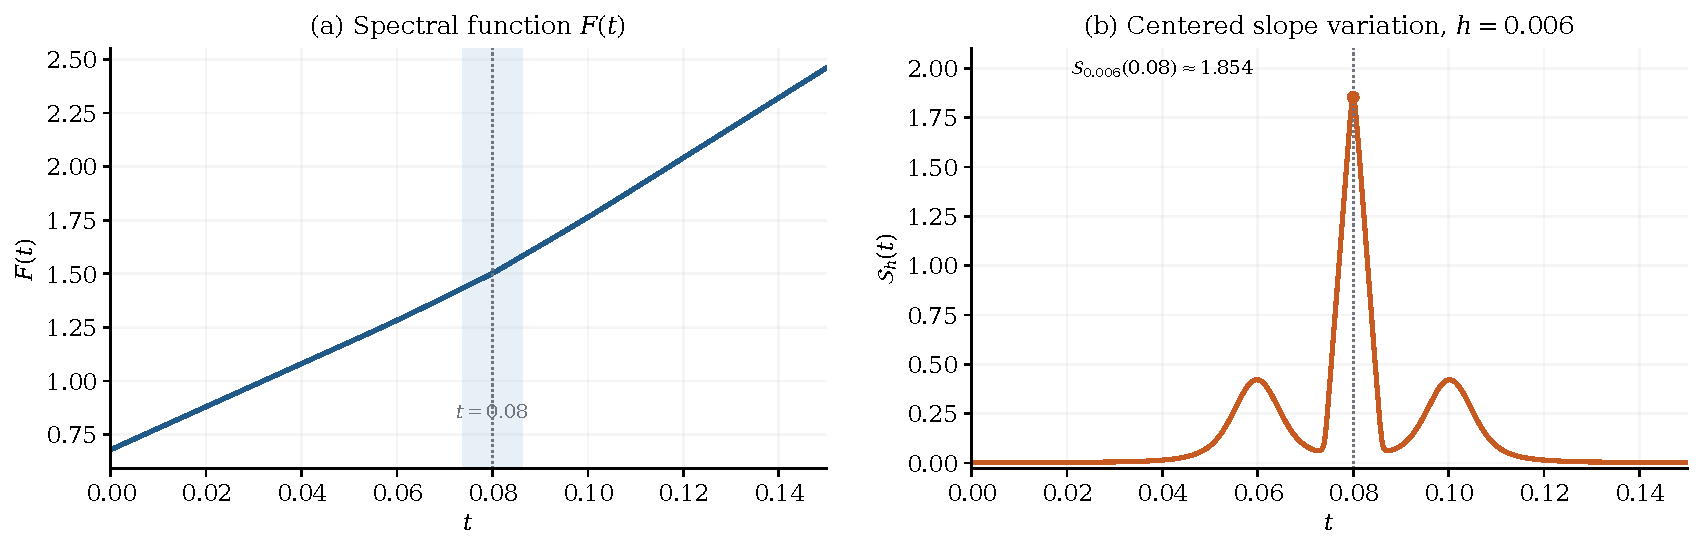
\includegraphics[width=0.98\linewidth]{ke02_tridiagonal_slope_variation_updated.pdf}
\caption{\Cref{ex:tridiagonal-defect} with $h=0.006$.
Left: the spectral function $F(t)$, with the
perturbation window highlighted around $t=0.08$.
Right: the corresponding centered slope variation
$\mathcal S_h(t)$, showing three smooth peaks.
At $t=0.08$, the slope variation is approximately
$1.8541$.}
\label{fig:tridiagonal-defect}
\end{figure}


\section{Small slope variation certifies a spectral gap}
\label{sec:local-gap}

The main result of this section shows that a sufficiently small centered
slope variation certifies a quantitative lower bound on the minimum
eigenvalue gap. We first state the certificate and then develop its two
ingredients: a localization argument that uses the tridiagonal structure,
and a stability argument that transfers the slope variation from a nearby
auxiliary matrix to the original perturbation family.

Throughout, fix $t\in[0,\delta/n]$ and write $H=H(t)=T+tX$ when the
parameter is fixed. We work in real symmetric coordinates by
\Cref{rem:real}; in particular, $\norm{H}_2\leq2$ and
$|H_{i,i+1}|\leq1$.

\begin{proposition}[Local gap certificate]\label{prop:bridge}
For $t\in[0,\delta/n]$ and $0<h\leq1$,
\begin{equation}\label{eq:bridge}
\boxed{\mathcal S_h(t)<\frac12\quad\Longrightarrow\quad
\gap(H(t))>\frac{h^2}{2^{20}n^4}.}
\end{equation}
\end{proposition}

We prove the contrapositive. A small eigenvalue gap forces two approximate
eigenvectors to be separated by a cut in the coordinate basis of $X$.
We then make them exact eigenvectors at a common eigenvalue of a nearby
matrix. Their distinct responses to $X$ force a slope variation of at
least one, and the perturbation error is too small to remove this signal.

\subsection{Localization: a near-degenerate pair splits across a cut}
\label{subsec:localization}

The key structural step is to construct two approximate eigenvectors whose
projections lie in disjoint coordinate subspaces. This is where the
tridiagonal assumption enters; note that the tridiagonal assumption is only used in this subsection. 
\Cref{ex:localization} illustrates how two nearby eigenvalues of a
tridiagonal matrix give rise to approximate eigenvectors
supported in disjoint coordinate subspaces, with
distinct responses to the diagonal perturbation.

\begin{example}[An illustrative example of a small-leakage cut]
\label{ex:localization}

Consider an $8\times8$ real symmetric tridiagonal matrix
\[
H=\diag(d_1,\ldots,d_8)
+\sum_{i=1}^7\beta_i
(e_ie_{i+1}^{\mathsf T}+e_{i+1}e_i^{\mathsf T}),
\]
where, with $\gamma=10^{-5}$,
\[
\begin{aligned}
(d_1,\ldots,d_8)
={}&
\left(\frac14-\frac\gamma2,\,
\frac12-\frac\gamma2,\,
\frac14-\frac\gamma2,\,
\frac12,\,\frac12,\,
\frac\gamma2,\,\frac\gamma2,\,\frac\gamma2\right),\\
(\beta_1,\ldots,\beta_7)
={}&
\left(-\frac14,-\frac14,0.0005,0.1,
0.0005,\frac14,\frac14\right).
\end{aligned}
\]
All off-diagonal entries are nonzero, and $\norm{H}_2<1$. 
Two eigenvalues are
$\lambda\approx-5.173792\times10^{-6}$ and
$\mu\approx4.739763\times10^{-6}$, satisfying
$|\lambda-\mu|<\gamma$.
Their corresponding orthonormal eigenvectors are
approximately
\[
\begin{aligned}
u_1&\approx(0.577344,0.577345,0.577346,-0.000602,
0.000123,-0.003033,-1.23\times10^{-7},0.003033)^{\mathsf T},\\
u_2&\approx(0.002477,0.002477,0.002477,0.000145,
-0.000736,0.707100,7.36\times10^{-7},-0.707100)^{\mathsf T}.
\end{aligned}
\]

We choose the cut $k=4$, separating the coordinate
subspaces $\spn\{e_1,\ldots,e_4\}$ and
$\spn\{e_5,\ldots,e_8\}$. 
We call $k=4$ a small-leakage cut. 
We obtain two orthonormal approximate eigenvectors
\[
\begin{aligned}
v_1&\approx(0.577350,0.577350,0.577351,-0.000601,
0,0,0,0)^{\mathsf T},\\
v_2&\approx(0,0,0,0,-0.000737,0.707107,
7.37\times10^{-7},-0.707107)^{\mathsf T}.
\end{aligned}
\]
Their coordinate supports are disjoint, and direct
computation gives
\[
\norm{\left(H-\frac{\lambda+\mu}{2}I\right)v_1}_2
\approx6.15\times10^{-5},\qquad
\norm{\left(H-\frac{\lambda+\mu}{2}I\right)v_2}_2
\approx7.53\times10^{-5}.
\]
Moreover, for $X=\diag(1,\ldots,8)$,
\[
v_2^{\mathsf T}Xv_2-v_1^{\mathsf T}Xv_1
\approx5.0000\geq1.
\]
\textbf{How do we obtain $v_1,v_2$?} We first construct two linear
combinations of the original eigenvectors $u_1,u_2$.
Choose $p=2$ and $q=6$, corresponding to two rows
with substantial norms and distinct directions,
on opposite sides of the cut. Write $r_i=((u_1)_i,(u_2)_i)\in\R^{1\times2}$ and define
\[
w_1=\frac{u_1[p]u_1+u_2[p]u_2}
{\sqrt{u_1[p]^2+u_2[p]^2}}=\frac{[u_1\ \ u_2]\,r_p^{\mathsf T}}{\norm{r_p}_2},
\qquad
w_2=\frac{u_1[q]u_1+u_2[q]u_2}
{\sqrt{u_1[q]^2+u_2[q]^2}}=\frac{[u_1\ \ u_2]\,r_q^{\mathsf T}}{\norm{r_q}_2},
\]
where $u_j[i]$ denotes the $i$th entry of $u_j$.
Let $P_L$ and $P_R$ be the orthogonal projections
onto $\spn\{e_1,\ldots,e_4\}$ and
$\spn\{e_5,\ldots,e_8\}$, respectively. We set
\[
v_1=\frac{P_Lw_1}{\norm{P_Lw_1}_2},
\qquad
v_2=\frac{P_Rw_2}{\norm{P_Rw_2}_2}.
\]
\end{example}

\begin{lemma}[Spatially separated approximate eigenvectors]
\label{lem:localization}
Suppose $\lambda,\mu$ are two eigenvalues of $H(t)$, counted with
multiplicity, satisfying $0\leq|\lambda-\mu|\leq\gamma\leq
1/(256n^2)$ with $\gamma>0$. Then there exist a cut $1\leq k<n$
and orthonormal unit vectors
$v_1\in\spn\{e_1,\ldots,e_k\}$ and
$v_2\in\spn\{e_{k+1},\ldots,e_n\}$ such that
\begin{equation}\label{eq:quasi}
\boxed{
\left\lVert\left(H(t)-\frac{\lambda+\mu}{2}I\right)v_i
\right\rVert_2\leq16n\sqrt\gamma\quad(i=1,2),
\qquad v_2^{\mathsf T}Xv_2-v_1^{\mathsf T}Xv_1\geq1.
}
\end{equation}
\end{lemma}

\begin{proof}
Fix $t$ and write $H=H(t)$. Choose orthonormal eigenvectors
$u_1,u_2$ associated with $\lambda,\mu$, respectively, and
write $r_i=((u_1)_i,(u_2)_i)\in\R^{1\times2}$.
By orthogonality, $\sum_{i=1}^n r_i^{\mathsf T}r_i=I_2$.

\emph{Step 1. Two substantial rows with separated directions.}
Let $J=\{i:\norm{r_i}_2\geq1/(2\sqrt n)\}$.
The discarded rows have total squared norm at most $1/4$.
Consequently,
$\sum_{i\in J}r_i^{\mathsf T}r_i\succeq(3/4)I_2$
and $\sum_{i\in J}\norm{r_i}_2^2\leq2$.

Choose any $p\in J$ and a unit vector $e\in\R^2$
perpendicular to $r_p$. Then
$\sum_{i\in J}|r_ie|^2\geq3/4$. Since
\[
\sum_{i\in J}|r_ie|^2
=\sum_{i\in J}\norm{r_i}_2^2\,
\frac{|r_ie|^2}{\norm{r_i}_2^2}
\qquad\text{and}\qquad
\sum_{i\in J}\norm{r_i}_2^2\leq2,
\]
the average of the ratios $|r_ie|^2/\norm{r_i}_2^2$,
$i\in J$, weighted by $\norm{r_i}_2^2$, is at least
$(3/4)/2=3/8$. Hence there exists $q\in J$ satisfying
$|r_qe|^2/\norm{r_q}_2^2\geq3/8$; in particular
$q\neq p$, since $r_pe=0$.
After exchanging $p,q$ if necessary, assume $p<q$.

For every nonzero row, let
$\Pi_i=r_i^{\mathsf T}r_i/\norm{r_i}_2^2$,
the rank-one orthogonal projector onto its direction.
Since
$\norm{\Pi_i-\Pi_j}_2
=|\det(r_i,r_j)|/(\norm{r_i}_2\norm{r_j}_2)$,
we obtain
\begin{equation}\label{eq:endpoints}
\boxed{
\norm{r_p}_2,\norm{r_q}_2\geq\frac1{2\sqrt n},
\qquad
\norm{\Pi_p-\Pi_q}_2\geq\sqrt{\frac38}>\frac12.
}
\end{equation}
Thus two rows have substantial norms but distinctly
different directions.

\emph{Step 2. Wronskian identity.}
Write $d_i=H_{ii}$ and $\beta_i=H_{i,i+1}$.
The eigenvector equations at coordinate $i$ are
\[
\begin{aligned}
\beta_{i-1}(u_1)_{i-1}+d_i(u_1)_i+\beta_i(u_1)_{i+1}
&=\lambda(u_1)_i,\\
\beta_{i-1}(u_2)_{i-1}+d_i(u_2)_i+\beta_i(u_2)_{i+1}
&=\mu(u_2)_i.
\end{aligned}
\]
Multiplying the first equation by $(u_2)_i$,
the second by $(u_1)_i$, subtracting, and summing
from $1$ to $i$ gives the discrete Wronskian identity
\begin{equation}\label{eq:wronskian}
\boxed{
\beta_i
\det\begin{pmatrix}
(u_1)_i&(u_1)_{i+1}\\
(u_2)_i&(u_2)_{i+1}
\end{pmatrix}
=
\beta_i\det\begin{pmatrix}r_i\\r_{i+1}\end{pmatrix}
=
(\mu-\lambda)\sum_{j=1}^i(u_1)_j(u_2)_j.
}
\end{equation}

Let $P_{\leq i}=\sum_{j=1}^i e_je_j^{\mathsf T}$.
Since $u_1^{\mathsf T}u_2=0$, Cauchy--Schwarz gives
\[
\left|\sum_{j=1}^i(u_1)_j(u_2)_j\right|
=
\left|u_1^{\mathsf T}
\left(P_{\leq i}-\frac12I\right)u_2\right|
\leq\frac12.
\]
Thus
$|\beta_i|\,|\det(r_i,r_{i+1})|\leq\gamma/2$.

\emph{Step 3. Finding a small-leakage cut.}
Set $\tau=4\sqrt{n\gamma}$. We claim that there exists
$p\leq k<q$ such that
\begin{equation}\label{eq:leak}
\boxed{
|\beta_k|\max\{\norm{r_k}_2,\norm{r_{k+1}}_2\}
\leq\tau.
}
\end{equation}
Suppose otherwise. Call a row \emph{large} if
$\norm{r_i}_2>\tau$, and \emph{small} otherwise.
Since $\tau\leq1/(4\sqrt n)$, the endpoint rows
$r_p,r_q$ are large.

We distinguish three cases.

\emph{(a) Two adjacent large rows.}
If $r_i,r_{i+1}$ are both large, the failure of
\eqref{eq:leak} implies
$|\beta_i|\norm{r_i}_2\norm{r_{i+1}}_2>\tau^2$.
The Wronskian bound therefore yields
\[
\norm{\Pi_i-\Pi_{i+1}}_2
=
\frac{|\det(r_i,r_{i+1})|}
{\norm{r_i}_2\norm{r_{i+1}}_2}
\leq\frac{\gamma}{2\tau^2}.
\]
Thus two adjacent large rows must have nearly
parallel directions.

\emph{(b) Two adjacent small rows.}
If both $r_i,r_{i+1}$ are small, then
$|\beta_i|\leq1$ gives
$|\beta_i|\max\{\norm{r_i}_2,\norm{r_{i+1}}_2\}
\leq\tau$, contradicting our assumption.
Hence small rows cannot occur consecutively.

\emph{(c) A large--small--large configuration.}
Suppose $r_{i-1},r_{i+1}$ are large but $r_i$
is small. The direction of $r_i$ itself need
not be well controlled, so we compare the
directions of $r_{i-1}$ and $r_{i+1}$ directly.

The three-term recurrence at row $i$ gives
\[
\beta_{i-1}r_{i-1}
+\left(d_i-\frac{\lambda+\mu}{2}\right)r_i
+\beta_ir_{i+1}
=
r_i\diag\left(\frac{\lambda-\mu}{2},
\frac{\mu-\lambda}{2}\right).
\]
Taking the determinant with $r_{i-1}$,
using the Wronskian bound and
$|d_i-(\lambda+\mu)/2|\leq4$, yields
\[
\norm{\Pi_{i-1}-\Pi_{i+1}}_2
\leq
\frac{2\gamma}
{|\beta_{i-1}\beta_i|
\norm{r_{i-1}}_2\norm{r_{i+1}}_2}
+
\frac{\gamma\norm{r_i}_2}
{2|\beta_i|\norm{r_{i+1}}_2}
\leq\frac{5\gamma}{\tau^2}.
\]
Indeed, the failure of \eqref{eq:leak} implies
$|\beta_{i-1}|\norm{r_{i-1}}_2>\tau$
and $|\beta_i|\norm{r_{i+1}}_2>\tau$,
while $\norm{r_i}_2\leq\tau\leq1$.
Hence the first term is less than $2\gamma/\tau^2$ and
the second is less than $\gamma/2$; moreover
$\gamma/2\leq3\gamma/\tau^2$ because
$\tau^2=16n\gamma\leq1/(16n)$.

We now follow the large rows from $p$ to $q$,
skipping any isolated small rows. By case~(b),
two successive large rows on this path are either
adjacent, as in case~(a), or separated by a single
small row, as in case~(c). The path therefore has
at most $q-p\leq n-1$ steps, each changing the
projector by at most
$5\gamma/\tau^2=5/(16n)$. By the triangle inequality
for the projector differences along the path,
the total change in direction satisfies
\[
\norm{\Pi_p-\Pi_q}_2
\leq(n-1)\frac{5\gamma}{\tau^2}
<\frac{5n\gamma}{\tau^2}
=\frac5{16}<\frac12.
\]
This contradicts \eqref{eq:endpoints}, proving
the existence of the cut \eqref{eq:leak}.

\emph{Step 4. Projection, truncation, and normalization.}
Using the row $r_p$, define the unit vector
\[
w_1=
\frac{(u_1)_p u_1+(u_2)_p u_2}{\norm{r_p}_2}.
\]
By construction, $(w_1)_p=\norm{r_p}_2$,
$|(w_1)_i|\leq\norm{r_i}_2$, and
$\left\lVert(H-\frac{\lambda+\mu}{2}I)w_1
\right\rVert_2\leq\gamma/2$.

Let $P_L=\sum_{i=1}^k e_ie_i^{\mathsf T}$
be the orthogonal projection onto the first
$k$ coordinate directions. Since $p\leq k$,
$\norm{P_Lw_1}_2\geq\norm{r_p}_2\geq1/(2\sqrt n)$.

By tridiagonality, the commutator
$[H,P_L]=HP_L-P_LH$ has only two boundary
contributions:
\[
[H,P_L]w_1
=\beta_k(w_1)_ke_{k+1}
-\beta_k(w_1)_{k+1}e_k.
\]
The small-leakage bound \eqref{eq:leak}
therefore gives
$\norm{[H,P_L]w_1}_2\leq\sqrt2\tau$.

Define $v_1=P_Lw_1/\norm{P_Lw_1}_2$.
Combining the residual and boundary estimates,
\[
\left\lVert
\left(H-\frac{\lambda+\mu}{2}I\right)v_1
\right\rVert_2
\leq2\sqrt n\left(\frac\gamma2+\sqrt2\tau\right)
\leq4\sqrt n\tau=16n\sqrt\gamma.
\]

Similarly, using the row $r_q$, define
$w_2=((u_1)_q u_1+(u_2)_q u_2)/\norm{r_q}_2$.
Let $P_R=\sum_{i=k+1}^n e_ie_i^{\mathsf T}$
and set $v_2=P_Rw_2/\norm{P_Rw_2}_2$.
The same argument gives
$\left\lVert(H-\frac{\lambda+\mu}{2}I)v_2
\right\rVert_2\leq16n\sqrt\gamma$.

The vectors $v_1,v_2$ have disjoint coordinate
supports and are therefore orthonormal.
Finally, since $X=\diag(1,\ldots,n)$,
$v_1^{\mathsf T}Xv_1\leq k$ and
$v_2^{\mathsf T}Xv_2\geq k+1$, proving
$v_2^{\mathsf T}Xv_2-v_1^{\mathsf T}Xv_1\geq1$.
\end{proof}

\begin{example}[Identifying the small-leakage cut in \Cref{ex:localization}]
\label{rem:localization-example}
Returning to \Cref{ex:localization}, write
$[u_1\ \ u_2]^{\mathsf T}=[r_1^{\mathsf T}\ \cdots\ r_8^{\mathsf T}]$,
where $r_i=((u_1)_i,(u_2)_i)$ as in the proof of \Cref{lem:localization}.
The determinant in \eqref{eq:wronskian} is the $2\times2$ minor
$\det[r_i^{\mathsf T}\ r_{i+1}^{\mathsf T}]$. The dashed vertical line below
marks the selected cut $k=4$, between columns $4$ and $5$.
\begin{equation}\label{eq:localization-row-minors}
\resizebox{0.91\linewidth}{!}{$\displaystyle
[u_1\ \ u_2]^{\mathsf T}=[r_1^{\mathsf T}\ \cdots\ r_8^{\mathsf T}]\approx
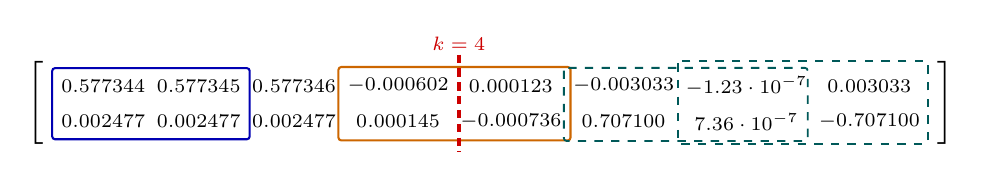
\begin{tikzpicture}[baseline=(M.center)]
\matrix (M) [matrix of math nodes,
 left delimiter={[},right delimiter={]},
 nodes={inner sep=1.6pt,anchor=center},
 column sep=1pt,row sep=3pt,font=\scriptsize] {
 0.577344 \pgfmatrixnextcell 0.577345 \pgfmatrixnextcell 0.577346 \pgfmatrixnextcell -0.000602 \pgfmatrixnextcell 0.000123 \pgfmatrixnextcell -0.003033 \pgfmatrixnextcell -1.23\cdot10^{-7} \pgfmatrixnextcell 0.003033 \\
 0.002477 \pgfmatrixnextcell 0.002477 \pgfmatrixnextcell 0.002477 \pgfmatrixnextcell 0.000145 \pgfmatrixnextcell -0.000736 \pgfmatrixnextcell 0.707100 \pgfmatrixnextcell 7.36\cdot10^{-7} \pgfmatrixnextcell -0.707100 \\
};
\draw[blue!70!black,line width=.75pt,rounded corners=1pt]
 ([xshift=-1.5pt,yshift=2.3pt]M-1-1.north west)
 rectangle ([xshift=1.5pt,yshift=-2.3pt]M-2-2.south east);
\draw[orange!80!black,line width=.75pt,rounded corners=1pt]
 ([xshift=-1.5pt,yshift=2.3pt]M-1-4.north west)
 rectangle ([xshift=1.5pt,yshift=-2.3pt]M-2-5.south east);
\draw[teal!70!black,dashed,line width=.65pt,rounded corners=1pt]
 ([xshift=-1.5pt,yshift=2pt]M-1-6.north west)
 rectangle ([xshift=1.5pt,yshift=-2pt]M-2-7.south east);
\draw[teal!70!black,dashed,line width=.65pt,rounded corners=1pt]
 ([xshift=-1pt,yshift=3.7pt]M-1-7.north west)
 rectangle ([xshift=1pt,yshift=-3.7pt]M-2-8.south east);
\coordinate (cutTop) at ($(M-1-4.north east)!0.5!(M-1-5.north west)$);
\coordinate (cutBottom) at ($(M-2-4.south east)!0.5!(M-2-5.south west)$);
\coordinate (cutBottomAligned) at (cutTop |- M-2-4.south);
\draw[red!80!black,densely dashed,line width=1.25pt]
 ([yshift=7pt]cutTop) -- ([yshift=-7pt]cutBottomAligned);
\node[red!80!black,above=5pt,font=\scriptsize] at (cutTop) {$k=4$};
\end{tikzpicture}.
$}
\end{equation}

For $\gamma=10^{-5}$ and $n=8$, the threshold is
$\tau=4\sqrt{n\gamma}\approx0.0358$. At any cut $k$,
we must check the \emph{leakage}
$L_k:=|\beta_k|\max\{\|r_k\|_2,\|r_{k+1}\|_2\}$,
not just the determinant of the two columns. The values of $L_k$ for all seven cuts are:
\[
\begin{array}{c|ccccccc}
 k&1&2&3&4&5&6&7\\ \hline
 \text{row types}&\mathrm{L-L}&\mathrm{L-L}&\mathrm{L-S}&\mathrm{S-S}&\mathrm{S-L}&\mathrm{L-S}&\mathrm{S-L}\\
 L_k&.1443&.1443&.000289&.0000746&.000354&.1768&.1768\\
 L_k\leq\tau?&\text{No}&\text{No}&\text{Yes}&\text{Yes}&\text{Yes}&\text{No}&\text{No}
\end{array}
\]
Here $\mathrm{L}$ and $\mathrm{S}$ indicate whether the row norm is
larger or smaller than $\tau$, respectively.

\emph{(a) Two adjacent large rows (blue box).}
At $k=1$, both columns have norms approximately $0.577$,
and $|\det[r_1^{\mathsf T}\ r_2^{\mathsf T}]|\approx5.67\times10^{-8}$.
Nevertheless, $L_1\approx0.1443>\tau$, so this is \emph{not}
a small-leakage cut. The columns are nearly parallel; this is
why a small Wronskian determinant alone does not produce the cut.

\emph{(b) Two adjacent small rows (orange box).}
At $k=4$, the column norms are approximately
$6.19\times10^{-4}$ and $7.46\times10^{-4}$.
Consequently, $L_4\approx7.46\times10^{-5}<\tau$.
Thus \emph{the orange block gives a valid cut}.
In fact, the adjacent cuts $k=3$ and $k=5$ also satisfy the
condition, owing to their small off-diagonal couplings.

\emph{(c) A large--small--large configuration (green boxes).}
The columns $r_6^{\mathsf T}$ and $r_8^{\mathsf T}$ have norms about $0.7071$,
while $\|r_7\|_2\approx7.46\times10^{-7}$.
Yet $L_6\approx L_7\approx0.1768>\tau$: neither adjacent
cut is valid. This is precisely why the contradiction argument
uses the three-term recurrence to compare the directions
of $r_6$ and $r_8$ directly, skipping the
intermediate small column.

The three cases are therefore not three ways of finding a cut.
They explain how the proof rules out the possibility that
\emph{every} cut has leakage greater than $\tau$.
The corresponding vectors are separated at the same cut:
\begin{equation}\label{eq:localization-vectors-cut}
\resizebox{0.91\linewidth}{!}{$\displaystyle
\begin{pmatrix}v_1^{\mathsf T}\\ v_2^{\mathsf T}\end{pmatrix}
\approx
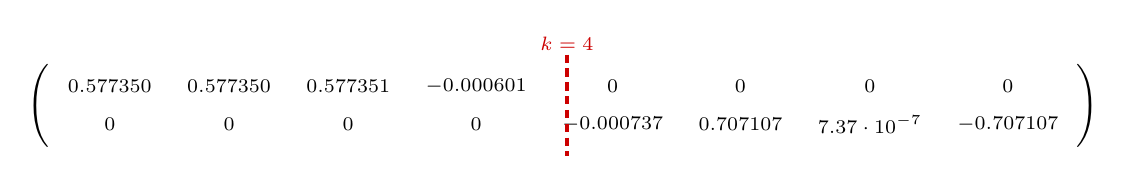
\begin{tikzpicture}[baseline=(V.center)]
\matrix (V) [matrix of math nodes,
 left delimiter={(},right delimiter={)},
 nodes={inner sep=1.9pt,anchor=center},
 column sep=9pt,row sep=4pt,font=\scriptsize] {
 0.577350 \pgfmatrixnextcell 0.577350 \pgfmatrixnextcell 0.577351 \pgfmatrixnextcell -0.000601 \pgfmatrixnextcell 0 \pgfmatrixnextcell 0 \pgfmatrixnextcell 0 \pgfmatrixnextcell 0 \\
 0 \pgfmatrixnextcell 0 \pgfmatrixnextcell 0 \pgfmatrixnextcell 0 \pgfmatrixnextcell -0.000737 \pgfmatrixnextcell 0.707107 \pgfmatrixnextcell 7.37\cdot10^{-7} \pgfmatrixnextcell -0.707107 \\
};
\coordinate (vCutTop) at ($(V-1-4.north east)!0.5!(V-1-5.north west)$);
\coordinate (vCutBottom) at ($(V-2-4.south east)!0.5!(V-2-5.south west)$);
\coordinate (vCutBottomAligned) at (vCutTop |- V-2-4.south);
\draw[red!80!black,densely dashed,line width=1.25pt]
 ([yshift=7pt]vCutTop) -- ([yshift=-7pt]vCutBottomAligned);
\node[red!80!black,above=5pt,font=\scriptsize] at (vCutTop) {$k=4$};
\end{tikzpicture}.
$}
\end{equation}

\end{example}



\paragraph{Where the structure enters.}
Only the localization lemma uses the tridiagonal recurrence:
through the Wronskian identity, the small-leakage cut, and the
boundary terms created by coordinate truncation. The rank-two
auxiliary construction and the nuclear-norm transfer apply to
general Hermitian matrices whenever appropriate approximate
eigenvectors with separated $X$-responses can be found.

\begin{remark}[Role of the tridiagonal structure]
\label{rem:tridiagonal-localization}
The tridiagonal assumption enters at three points:
the discrete Wronskian identity, the three-term
recurrence used to control directions across an
intermediate small row, and the two boundary terms
created by truncation at a cut. The initial
orthogonality argument and the projection onto
coordinate subspaces are not specific to
tridiagonal matrices.

Thus the structural role of tridiagonality is
to guarantee a cut with small boundary leakage.
Once the approximate eigenvectors in
\Cref{lem:localization} have been constructed,
the auxiliary-matrix argument and the subsequent
slope-variation estimates do not require the
auxiliary matrix to remain tridiagonal.
\end{remark}

\subsection{From the cut to the gap certificate}
\label{subsec:gap-transfer}

The preceding lemma is the only step that uses the tridiagonal
recurrence. We now replace the two localized approximate eigenvectors
by exact eigenvectors with a common eigenvalue in a nearby auxiliary
matrix. This gives a uniform slope response, which we then transfer
back to the original family.

\begin{lemma}[A nearby matrix with large slope variation]
\label{lem:auxiliary}
Under the assumptions of \Cref{lem:localization}, there is a real
symmetric matrix $\widetilde H$ for which
\begin{equation}\label{eq:auxiliary}
\boxed{\widetilde Hv_i=\frac{\lambda+\mu}{2}v_i\quad(i=1,2),
\qquad\norm{H(t)-\widetilde H}_*\leq96n\sqrt\gamma,}
\end{equation}
where $\|\cdot\|_*$ denotes the nuclear norm. 
The nuclear-norm bound measures its distance from
$H(t)$ and will allow us to transfer the slope-variation
estimate back to the original perturbation family. The auxiliary matrix is not required to be tridiagonal.
Define $\widetilde H(s)=\widetilde H+(s-t)X$ and
$F^{\mathrm{aux}}(s)=\sum_{j=1}^n j\lambda_j(\widetilde H(s))$.
Then the centered slope variation of the auxiliary family satisfies
\begin{equation}\label{eq:auxiliary-defect}
\boxed{\mathcal S_h^{\mathrm{aux}}(t)
:=\frac{F^{\mathrm{aux}}(t+h)+F^{\mathrm{aux}}(t-h)
-2F^{\mathrm{aux}}(t)}{h}\geq1\qquad(h>0).}
\end{equation}
\end{lemma}

\begin{proof}
Take $v_1,v_2$ from \Cref{lem:localization} and set
$Q=v_1v_1^{\mathsf T}+v_2v_2^{\mathsf T}$ and
$\widetilde H=(I-Q)H(t)(I-Q)+(\lambda+\mu)Q/2$.
Because $Qv_i=v_i$, both are exact eigenvectors of
$\widetilde H$ at the common eigenvalue $(\lambda+\mu)/2$.
Moreover, expanding $H(t)-\widetilde H$ gives
\[
H(t)-\widetilde H
=\bigl(H(t)-\tfrac{\lambda+\mu}{2}I\bigr)Q
+Q\bigl(H(t)-\tfrac{\lambda+\mu}{2}I\bigr)
-Q\bigl(H(t)-\tfrac{\lambda+\mu}{2}I\bigr)Q.
\]
Write $A=H(t)-\tfrac{\lambda+\mu}{2}I$, so that
$H(t)-\widetilde H=AQ+QA-QAQ$ with $A$ real symmetric.
Since $Q$ is an orthogonal projector of rank two, $AQ$ has
rank at most two and
$\norm{AQ}_{\mathrm F}^2=\tr(QA^2Q)
=\sum_{i=1}^2\norm{Av_i}_2^2$.
The nuclear--Frobenius norm inequality for matrices of rank
at most two gives $\norm{AQ}_*\leq\sqrt2\norm{AQ}_{\mathrm F}$.
Moreover, $QA=(AQ)^{\mathsf T}$ has the same singular values
as $AQ$, and $QAQ=Q(AQ)$ has rank at most two and
$\norm{QAQ}_{\mathrm F}\leq\norm{AQ}_{\mathrm F}$. Hence
\[
\norm{AQ}_*,\ \norm{QA}_*,\ \norm{QAQ}_*
\leq\sqrt2\norm{AQ}_{\mathrm F}.
\]
The triangle inequality and \eqref{eq:quasi} yield
\[
\norm{H(t)-\widetilde H}_*
\leq3\sqrt2\left(\sum_{i=1}^2
\norm{Av_i}_2^2
\right)^{1/2}
\leq3\sqrt2\cdot\sqrt2\cdot16n\sqrt\gamma
=96n\sqrt\gamma.
\]

For the slope variation, choose an ordered orthonormal eigenbasis
of $\widetilde H$ in which $v_1,v_2$ occupy adjacent places
$j,j+1$ in their common eigenspace. Assign the corresponding
weights $j,j+1$ first to $v_1,v_2$, then in the opposite order.
Both choices maximize the variational representation
\eqref{eq:variational} at $s=t$. The corresponding matrices
$G_+,G_-$ satisfy
\[
\tr(G_+\widetilde H)=\tr(G_-\widetilde H)=F^{\mathrm{aux}}(t),
\qquad G_+-G_-=v_2v_2^{\mathsf T}-v_1v_1^{\mathsf T}.
\]
Using $G_+$ at $t+h$ and $G_-$ at $t-h$ gives
\[
\mathcal S_h^{\mathrm{aux}}(t)
\geq\tr\bigl((G_+-G_-)X\bigr)
=v_2^{\mathsf T}Xv_2-v_1^{\mathsf T}Xv_1\geq1.
\]
\end{proof}

\begin{proof}[Proof of \Cref{prop:bridge}]
We prove the contrapositive. Suppose
$\gap(H(t))\leq\gamma:=h^2/(2^{20}n^4)$.
Because $0<h\leq1$, we have $0<\gamma\leq1/(256n^2)$.
Choose two eigenvalues $\lambda,\mu$ realizing the minimum gap,
including $\lambda=\mu$ if the gap is zero. By
\Cref{lem:localization,lem:auxiliary}, we have
$\norm{H(t)-\widetilde H}_*\leq96n\sqrt\gamma$ and
$\mathcal S_h^{\mathrm{aux}}(t)\geq1$.

By the variational representation \eqref{eq:variational}
and operator--nuclear norm duality, for every $s$,
\begin{equation}\label{eq:nuclear}
\boxed{
|F(s)-F^{\mathrm{aux}}(s)|
\leq n\norm{H(s)-\widetilde H(s)}_*
=n\norm{H(t)-\widetilde H}_*.
}
\end{equation}
The original and auxiliary families differ by the constant matrix
$H(t)-\widetilde H$, since
$H(s)-\widetilde H(s)=H(t)-\widetilde H$ for all $s$.
Applying \eqref{eq:nuclear} at $t-h,t,t+h$ yields
\[
\mathcal S_h(t)\geq\mathcal S_h^{\mathrm{aux}}(t)
-\frac{4n}{h}\norm{H(t)-\widetilde H}_*
\geq1-\frac{384n^2\sqrt\gamma}{h}.
\]
At $\gamma=h^2/(2^{20}n^4)$, the right-hand side equals
$1-384/1024=5/8>1/2$, proving \eqref{eq:bridge}.
\end{proof}

\section{The algorithm: adaptive selection of the perturbation parameter}
\label{sec:selection}

The purpose of this section is to construct a diagonal
perturbation $D=tX$ that guarantees quantitative spectral
separation. By \Cref{prop:bridge}, it suffices to find
a parameter $t$ and a window radius $h$ such that
\[
\mathcal S_h(t)<\frac12
\quad\Longrightarrow\quad
\gap(H(t))>\frac{h^2}{2^{20}n^4}.
\]
The key observation is that the convex spectral function
$F$ has a bounded total increase in slope. Although its
slope may vary rapidly over some windows, repeated interval
refinement allows us to find a window with sufficiently
small slope variation.


We first establish a simple interval-selection algorithm
and then improve its contraction and the resulting gap
bound. Both algorithms check the local certificate at
each selected window and terminate as soon as it is
verified. We prove explicit worst-case iteration bounds
and finally explain how the required spectral-function
evaluations can be carried out efficiently.



\subsection{A basic selector}
\label{subsec:basic-selection}

We represent each interval by $I=[t-h,t+h]$,
where $t$ is its center and $h$ is its radius.
At each iteration, we compare the centered slope
variations on the two middle subintervals
\[
I_{\mathrm L}=[t-h/2,t],
\qquad
I_{\mathrm R}=[t,t+h/2].
\]
Their centers are $t-h/4$ and $t+h/4$, respectively,
and both have radius $h/4$.


The basic procedure selects the subinterval with
smaller computed slope variation. At each iteration,
we also check whether the selected window already
satisfies the local gap certificate. We will show
that the algorithm must terminate after at most
$O(\log n)$ refinements, while maintaining an
inverse-polynomial lower bound on the window radius.


\begin{algorithm}[t]

\caption{Basic selection of a perturbation parameter}
\label{alg:selection-basic}
\DontPrintSemicolon
\KwIn{$T$, $n\geq2$, and $0<\delta<1/2$.}
\KwOut{A perturbation parameter $t$ and radius $h$.}

Set $t=\delta/(2n)$ and $h=\delta/(2n)$\;
Find the smallest nonnegative integer $K_{\mathrm b}$
with $(3/2)^{K_{\mathrm b}}\geq16n^3$ by repeated
multiplication by $3/2$ and comparisons\;

Evaluate $F(t-h)$, $F(t)$, and $F(t+h)$
to absolute error at most $h/256$\;
\If{$\widehat{\mathcal S}_h(t)+1/64<1/2$}{
    \Return{$t,h$}\;
}

\For{$j=0,\ldots,K_{\mathrm b}-1$}{
    Set $h=h/4$\;
    Evaluate $F$ at $t-2h,t-h,t,t+h,t+2h$
    to absolute error at most $h/256$\;
    Compute $\widehat{\mathcal S}_h(t-h)$ and
    $\widehat{\mathcal S}_h(t+h)$\;
    \eIf{$\widehat{\mathcal S}_h(t-h)
    \leq\widehat{\mathcal S}_h(t+h)$}{
        Set $t=t-h$\;
    }{
        Set $t=t+h$\;
    }
    \If{$\widehat{\mathcal S}_h(t)+1/64<1/2$}{
        \Return{$t,h$}\;
    }
}
(This line is not reached, by \Cref{thm:selection-basic}.)\;
\end{algorithm}

\begin{example}[One step of interval selection]
\label{ex:selection}
Consider the spectral function in \Cref{ex:collision},
whose centered slope variation is
\[
\mathcal S_h(t)
=\max\left\{1-\frac{|t-0.1|}{h},0\right\}.
\]
Starting with the illustrative window
$[0.06,0.14]$, centered at $t=0.1$ with $h=0.04$,
we have $\mathcal S_{0.04}(0.1)=1$.

After one refinement, the two candidate windows
are $[0.08,0.10]$ and $[0.10,0.12]$, with centers
$0.09$ and $0.11$ and radius $0.01$. Since $F$
is affine on each window,
\[
\mathcal S_{0.01}(0.09)
=\mathcal S_{0.01}(0.11)=0.
\]
Thus either candidate already satisfies
$\mathcal S_h(t)<1/2$.
More generally, the algorithm selects the candidate
with smaller slope variation, moving towards a
window where the spectral response is more stable.
\end{example}


We next combine the exact contraction property
of centered slope variation with the effect of
approximate spectral-function evaluations.



\begin{lemma}[Contraction of centered slope variation]
\label{lem:defect-contraction}
\label{lem:inexact-contraction}
For a parent interval $I=[t-h,t+h]$, let
$I_{\mathrm L}=[t-h/2,t]$ and
$I_{\mathrm R}=[t,t+h/2]$ be its two middle
subintervals. Then
\begin{equation}\label{eq:defect-contraction}
\boxed{
\min\left\{
\mathcal S_{h/4}\left(t-\frac h4\right),
\mathcal S_{h/4}\left(t+\frac h4\right)
\right\}
\leq\frac23\mathcal S_h(t).
}
\end{equation}
Moreover, if each value of $F$ is evaluated with
absolute error at most one 256th of the child
radius, the selected center and radius satisfy,
for every refinement $j$ of \Cref{alg:selection-basic}
that is performed,
\begin{equation}\label{eq:inexact-contraction}
\boxed{
\mathcal S_{h_{j+1}}(t_{j+1})
\leq
\frac23\mathcal S_{h_j}(t_j)+\frac1{32}.
}
\end{equation}
\end{lemma}

\begin{proof}
Recall from \eqref{eq:slope-curvature} that
the centered slope variation is a triangularly
weighted integral of $F''$ whenever $F$ is
twice continuously differentiable. For general
convex $F$, the same representation holds with
its distributional second derivative interpreted
as a nonnegative measure $\nu$.

Thus
\[
\mathcal S_h(t)
=\int_{\mathbb R}w_{t,h}(x)\,d\nu(x),
\qquad
w_{t,h}(x)=
\left(1-\frac{|x-t|}{h}\right)_+.
\]
A direct comparison of the triangular weights gives
\[
w_{t-h/4,h/4}(x)+w_{t+h/4,h/4}(x)
\leq\frac43w_{t,h}(x).
\]
Integrating against the nonnegative measure $\nu$
and taking half the sum proves
\eqref{eq:defect-contraction}.

For approximate evaluations, let $r=h/4$
be the child radius. Since the centered slope
variation uses the coefficients $1,-2,1$,
evaluating each of its three function values
within $r/256$ gives
\[
\left|
\widehat{\mathcal S}_r(s)
-\mathcal S_r(s)
\right|
\leq
\frac{(1+2+1)(r/256)}r
=\frac1{64}.
\]
Selecting the smaller computed child variation
therefore incurs an additional error of at most
$2/64=1/32$. Combining this estimate with
\eqref{eq:defect-contraction} proves
\eqref{eq:inexact-contraction}.
\end{proof}


\begin{figure}[h]
\centering
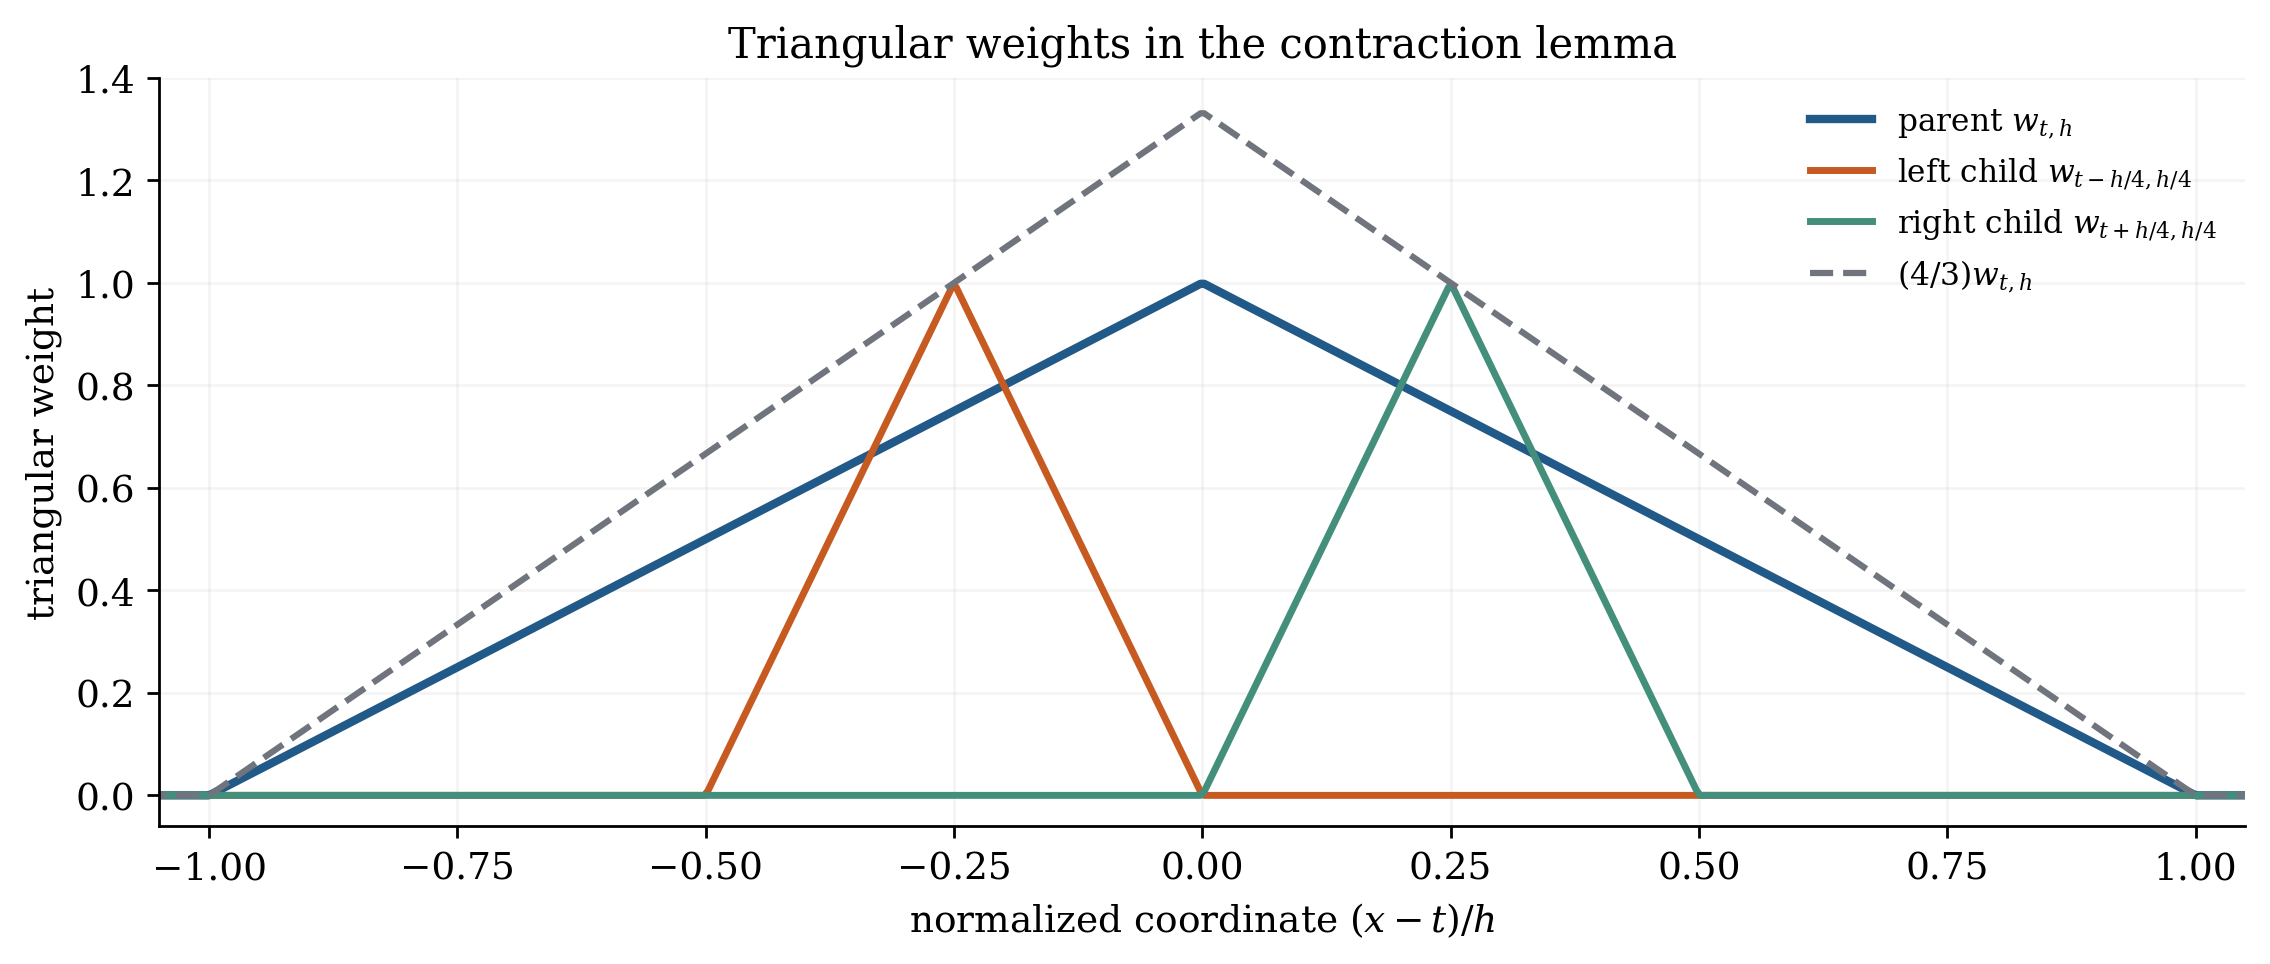
\includegraphics[width=0.86\linewidth]{ke02_triangular_weights.png}
\caption{Triangular weights for
\Cref{lem:defect-contraction}, plotted in the normalized
coordinate $(x-t)/h$. The two child weights correspond
to the middle subintervals $[t-h/2,t]$ and
$[t,t+h/2]$. Their sum is bounded pointwise by
$(4/3)$ times the parent weight.}
\label{fig:triangular-weights}
\end{figure}


The contraction estimate guarantees that the
slope variation eventually becomes small enough
for the certified stopping test. We now bound
the number of required refinements.



\begin{theorem}[Basic iteration bound and certified scale]
\label{thm:selection-basic}
Algorithm~\ref{alg:selection-basic} terminates after
at most
\[
K_{\mathrm b}
=\left\lceil\log_{3/2}(16n^3)\right\rceil
=O(\log n)
\]
refinements and returns $t,h$ satisfying
\begin{equation}\label{eq:selection-basic-output}
\boxed{
[t-h,t+h]\subseteq[0,\delta/n],
\qquad
\mathcal S_h(t)<\frac12,
\qquad
h\geq\frac{\delta}{2n}4^{-K_{\mathrm b}}.
}
\end{equation}
It requires at most $3+5K_{\mathrm b}$
spectral-function evaluations.

Consequently, the returned perturbation $D=tX$
satisfies $\norm D_2\leq\delta$ and
\[
\boxed{
\gap(T+D)>\frac{h^2}{2^{20}n^4}.
}
\]
\end{theorem}

\begin{proof}
Initially $t_0=h_0=\delta/(2n)$, so the initial
interval is $[0,\delta/n]$. Each refinement
selects a subinterval contained in its parent,
with radius one quarter of the parent radius.
Thus, if the algorithm stops after $j$
refinements,
\[
h_j=\frac{\delta}{2n}4^{-j},
\qquad
0\leq j\leq K_{\mathrm b}.
\]

By the secant-slope bounds in \Cref{lem:convex},
the initial slope variation satisfies
$\mathcal S_{h_0}(t_0)<n^3$.
Iterating \eqref{eq:inexact-contraction} gives
\[
\mathcal S_{h_j}(t_j)
<
\left(\frac23\right)^j n^3
+\frac1{32}\sum_{\ell=0}^{j-1}
\left(\frac23\right)^\ell
<
\left(\frac23\right)^j n^3+\frac3{32}.
\]
At $j=K_{\mathrm b}$, the first term is at
most $1/16$, so
\[
\mathcal S_{h_{K_{\mathrm b}}}
(t_{K_{\mathrm b}})
<\frac5{32}.
\]

Every computed slope variation has absolute
error at most $1/64$. Consequently, at the
$K_{\mathrm b}$th refinement,
\[
\widehat{\mathcal S}_{h_{K_{\mathrm b}}}
(t_{K_{\mathrm b}})
+\frac1{64}
<
\frac5{32}+\frac2{64}
<\frac12.
\]
Hence the certified stopping test must succeed
by this iteration. If it succeeds earlier,
the returned window is larger.

The initial test uses three evaluations of $F$,
and each refinement uses at most five.
Finally, $\norm{tX}_2=nt\leq\delta$, and since
$h\leq\delta/(2n)<1$, \Cref{prop:bridge} gives the claimed gap bound.
\end{proof}


\begin{remark}[A lower bound on the window radius]
\label{rem:basic-selection-scale}
Although the algorithm repeatedly reduces the window
radius, it performs only $O(\log n)$ refinements.
Let $\alpha=\log_{3/2}4$. By the minimality of
$K_{\mathrm b}$,
\begin{equation}\label{eq:basic-selection-scale}
\boxed{
h>\frac{\delta}{8n}(16n^3)^{-\alpha}.
}
\end{equation}
Thus the window radius remains bounded below by
an inverse polynomial in $n$. The next subsection
improves this bound by retaining longer intervals
at each refinement.
\end{remark}

\subsection{An improved selector that keeps almost half of each window}
\label{subsec:improved-selection}

The basic algorithm is simple, but each iteration retains only one quarter
of the parent interval. Since the local gap certificate depends on $h^2$,
this repeated reduction leads to a conservative bound. We now improve
the selection rule while keeping the spectral function $F$ and the local
certificate of \Cref{prop:bridge} unchanged. By comparing slopes near the
endpoints, we can retain almost half of the parent interval at each iteration.

\paragraph{Endpoint slope variation.}
For a window $I=[t-h,t+h]$ and $0<\theta\leq1/2$, define
\begin{equation}\label{eq:endpoint-slope}
\boxed{
\mathcal S_h^{(\theta)}(t)
:=
\frac{F(t+h)-F(t+(1-2\theta)h)}{2\theta h}
-
\frac{F(t-(1-2\theta)h)-F(t-h)}{2\theta h}.
}
\end{equation}
This measures the difference between the secant slopes near the two
endpoints and is nonnegative by convexity.


The endpoint slopes also control the centered slope variation. Indeed,
for $0<\theta\leq1/2$, convexity gives
\[
\frac{F(t-h+2\theta h)-F(t-h)}{2\theta h}
\leq\frac{F(t)-F(t-h)}h,
\qquad
\frac{F(t+h)-F(t)}h
\leq\frac{F(t+h)-F(t+h-2\theta h)}{2\theta h}.
\]
Subtracting yields
\begin{equation}\label{eq:potential-controls-S}
\boxed{\mathcal S_h(t)\leq\mathcal S_h^{(\theta)}(t).}
\end{equation}
Thus endpoint slope variation can be used for selection, while the
stopping test remains the original condition $\mathcal S_h(t)<1/2$.


Let $K=\lceil\log_2(16n^3)\rceil$ and $\theta=1/(4K)$.
For a current interval $I=[t-h,t+h]$, consider
\[
I_{\mathrm L}=[t-(1-2\theta)h,t],
\qquad
I_{\mathrm R}=[t,t+(1-2\theta)h].
\]
Both candidates have radius $h'=(1/2-\theta)h$, rather than $h/4$
as in the basic algorithm.

\begin{algorithm}[t]

\caption{Improved selection of a separating perturbation}
\label{alg:selection}
\DontPrintSemicolon
\KwIn{$T$, $n\geq2$, and $0<\delta<1/2$.}
\KwOut{A perturbation parameter $t$ and certification radius $h$.}

Find $K=\lceil\log_2(16n^3)\rceil$, the least integer
with $2^K\geq16n^3$, by doubling and comparisons, and
set $\theta=1/(4K)$\;
Set $t=\delta/(2n)$ and $h=\delta/(2n)$\;
Evaluate $F(t-h),F(t),F(t+h)$ to absolute error at most $h/256$\;
\If{$\widehat{\mathcal S}_h(t)+1/64<1/2$}{
    \Return{$t,h$}\;
}

\For{$j=0,\ldots,K-1$}{
    Set $h=(1/2-\theta)h$\;
    Evaluate the values of $F$ required for
    $\mathcal S_h^{(\theta)}(t-h)$ and
    $\mathcal S_h^{(\theta)}(t+h)$, each to absolute
    error at most $2\theta h/256$\;
    Compute $\widehat{\mathcal S}_h^{(\theta)}(t-h)$
    and $\widehat{\mathcal S}_h^{(\theta)}(t+h)$\;
    \eIf{$\widehat{\mathcal S}_h^{(\theta)}(t-h)
       \leq\widehat{\mathcal S}_h^{(\theta)}(t+h)$}{
        Set $t=t-h$\;
    }{
        Set $t=t+h$\;
    }
    Evaluate the additional midpoint value $F(t)$
    to absolute error at most $2\theta h/256$\;
    Compute $\widehat{\mathcal S}_h(t)$\;
    \If{$\widehat{\mathcal S}_h(t)+1/64<1/2$}{
        \Return{$t,h$}\;
    }
}
(This line is not reached, by \Cref{thm:selection}.)\;
\end{algorithm}


The following lemma is the endpoint analogue of
\Cref{lem:defect-contraction}. It combines the exact contraction
and the effect of approximate evaluations.

\begin{lemma}[Contraction of endpoint slope variation]
\label{lem:potential-contraction}
\label{lem:potential-inexact}
Let $I=[t-h,t+h]$, $h'=(1/2-\theta)h$, and
$0<\theta\leq1/4$. Then
\begin{equation}\label{eq:potential-contraction}
\boxed{
\min\left\{
\mathcal S_{h'}^{(\theta)}(t-h'),
\mathcal S_{h'}^{(\theta)}(t+h')
\right\}
\leq\frac12\mathcal S_h^{(\theta)}(t).
}
\end{equation}
Moreover, the selected centers and radii of
\Cref{alg:selection} satisfy
\begin{equation}\label{eq:potential-inexact-contraction}
\boxed{
\mathcal S_{h_{j+1}}^{(\theta)}(t_{j+1})
\leq\frac12\mathcal S_{h_j}^{(\theta)}(t_j)+\frac1{32}.
}
\end{equation}
\end{lemma}

\begin{proof}
As in \Cref{lem:defect-contraction}, convexity gives a contraction
between the parent and its two candidate windows. Here the endpoint
secants are ordered, and the two child slope differences correspond
to disjoint increments between the parent endpoint slopes.
Explicitly, write $\sigma[x,y]=(F(y)-F(x))/(y-x)$ for $x<y$.
By convexity, $\sigma[x,y]\leq\sigma[x',y']$ whenever
$x\leq x'$ and $y\leq y'$. Since $2h'=(1-2\theta)h$, the
parent endpoint secants are taken over
$[t-h,t-2h']$ and $[t+2h',t+h]$, the endpoint secants of
the left candidate over $[t-2h',t-2h'+2\theta h']$ and
$[t-2\theta h',t]$, and those of the right candidate over
$[t,t+2\theta h']$ and $[t+2h'-2\theta h',t+2h']$. Hence
\[
\sigma[t-h,t-2h']\leq\sigma[t-2h',t-2h'+2\theta h'],
\quad
\sigma[t-2\theta h',t]\leq\sigma[t,t+2\theta h'],
\quad
\sigma[t+2h'-2\theta h',t+2h']\leq\sigma[t+2h',t+h],
\]
that is, the left endpoint slope of the parent is at most
that of the left candidate, the right endpoint slope of the
left candidate is at most the left endpoint slope of the right
candidate, and the right endpoint slope of the right candidate
is at most that of the parent. Therefore
\[
\begin{aligned}
\mathcal S_{h'}^{(\theta)}(t-h')
+\mathcal S_{h'}^{(\theta)}(t+h')
&=\bigl(\sigma[t-2\theta h',t]-\sigma[t-2h',t-2h'+2\theta h']\bigr)\\
&\quad+\bigl(\sigma[t+2h'-2\theta h',t+2h']-\sigma[t,t+2\theta h']\bigr)\\
&\leq\sigma[t+2h',t+h]-\sigma[t-h,t-2h']
=\mathcal S_h^{(\theta)}(t).
\end{aligned}
\]
Both child variations are nonnegative, so the smaller one is at
most half of this sum, which proves \eqref{eq:potential-contraction}.

The inexact estimate follows as in the proof of
\Cref{lem:defect-contraction}. Each endpoint slope variation
uses four evaluations of $F$ with denominator $2\theta h_{j+1}$.
The prescribed absolute error $2\theta h_{j+1}/256$
therefore gives an error of at most $1/64$ in each
computed variation. Selecting the smaller computed value
adds at most $2/64=1/32$, proving
\eqref{eq:potential-inexact-contraction}.
\end{proof}



\begin{theorem}[Improved constructive spectral separation]
\label{thm:selection}
Algorithm~\ref{alg:selection} terminates after at most
\[
K=\left\lceil\log_2(16n^3)\right\rceil=O(\log n)
\]
refinements and returns $t,h$ satisfying
\begin{equation}\label{eq:selection-output}
\boxed{
[t-h,t+h]\subseteq[0,\delta/n],
\qquad
\mathcal S_h(t)<\frac12,
\qquad h>\frac{\delta}{128n^4}.
}
\end{equation}
Consequently, $D=tX$ satisfies
\begin{equation}\label{eq:selection-gap}
\boxed{
\norm D_2\leq\delta,\qquad
\gap(T+D)>2^{-34}\frac{\delta^2}{n^{12}}.
}
\end{equation}
The algorithm requires at most $3+8K$ spectral-function evaluations.
\end{theorem}

\begin{proof}
The argument follows that of \Cref{thm:selection-basic}, with
two improvements: the contraction factor is $1/2$ instead of
$2/3$, and each refinement retains a fraction $1/2-\theta$
rather than $1/4$ of the parent radius.

By \Cref{lem:convex} and
\eqref{eq:potential-inexact-contraction},
\[
\mathcal S_{h_K}^{(\theta)}(t_K)
\leq 2^{-K}n^3+\frac1{32}\sum_{j=0}^{K-1}2^{-j}
<\frac18.
\]
By \eqref{eq:potential-controls-S}, we also have
$\mathcal S_{h_K}(t_K)<1/8$. The endpoint values and
the additional midpoint evaluation give
\[
\left|\widehat{\mathcal S}_{h_K}(t_K)
-\mathcal S_{h_K}(t_K)\right|
\leq\frac{\theta}{32}\leq\frac1{128}.
\]
Thus $\widehat{\mathcal S}_{h_K}(t_K)+1/64<1/2$,
so the certified stopping test succeeds by iteration $K$.

Each candidate window $[t-(1-2\theta)h,t]$ or
$[t,t+(1-2\theta)h]$ is contained in its parent
$[t-h,t+h]$, and the initial window is $[0,\delta/n]$.
Hence the returned window satisfies
$[t-h,t+h]\subseteq[0,\delta/n]$, and every point at
which $F$ is evaluated lies in $[0,\delta/n]$.

It remains to bound the radius. As in
\Cref{thm:selection-basic}, termination at an earlier
iteration only increases the returned radius. Since
\[
L_K=\frac{\delta}{n}
\left(\frac12-\theta\right)^K
=\frac{\delta}{n}2^{-K}
\left(1-\frac1{2K}\right)^K
>\frac{\delta}{64n^4},
\]
where we used Bernoulli's inequality and $2^K<32n^3$,
the returned radius satisfies
$h\geq L_K/2>\delta/(128n^4)$.
Since also $h\leq\delta/(2n)<1$, applying \Cref{prop:bridge} yields
\[
\gap(T+tX)>
\frac{h^2}{2^{20}n^4}
>2^{-34}\frac{\delta^2}{n^{12}}.
\]
Finally, the initial test uses three evaluations of $F$.
In a refinement with updated radius $h$ and previous
center $t$, the two endpoint slope variations
$\mathcal S_h^{(\theta)}(t\mp h)$ use the values of $F$
at the seven points $t-2h$, $t-2h+2\theta h$, $t-2\theta h$,
$t$, $t+2\theta h$, $t+2h-2\theta h$, $t+2h$, where the
shared point $t$ is evaluated once. The stopping test at
the new center $t\mp h$ uses two of these values and the
additional midpoint value $F(t\mp h)$. Hence each refinement
uses at most eight evaluations.
\end{proof}

\begin{remark}[Improvement over the basic selector]
\label{rem:selection-scale}
Compared with \Cref{alg:selection-basic}, the improved selector
achieves a contraction factor of $1/2$ while retaining almost
half of the parent interval. Both algorithms use the same
centered-slope stopping test and the same local gap certificate.
The larger retained radius gives the stronger $n^{-12}$ bound
in \eqref{eq:selection-gap}, without changing the localization
argument of \Cref{sec:local-gap}.
\end{remark}


\subsection{Evaluating the spectral function in nearly linear time}
\label{subsec:oracle}

We finally explain how the required values of $F$
can be computed without treating an eigendecomposition
as a unit-cost operation. Both selection algorithms
use the same spectral-function oracle; the improved
selector changes only the evaluation points and
their required absolute accuracy.

For the tridiagonal family $H(t)=T+tX$, the
characteristic polynomial can be computed using
the three-term determinant recurrence.
Balanced polynomial multiplication and Graeffe
root-squaring then provide approximations to
the ordered eigenvalues. The algebraic details
are given in \Cref{app:oracle}.

\begin{lemma}[Spectral-function oracle]
\label{lem:oracle}
For $H(t)=T+tX$, $0\leq t\leq\delta/n$,
and any $0<\varepsilon<1$, one can compute
$\widehat F(t)$ satisfying
\begin{equation}\label{eq:oracle}
\boxed{
|\widehat F(t)-F(t)|\leq\varepsilon
}
\end{equation}
using
$O(n[1+\log(n/\varepsilon)]^2)$
exact arithmetic operations and comparisons,
where nonnegative square roots are permitted.
\end{lemma}

\begin{proof}
The construction uses the tridiagonal determinant
recurrence, balanced polynomial multiplication,
and Graeffe root-squaring. We refer to
\Cref{app:oracle} for the details; its cost is
accounted for as follows. Let
$\eta=2\varepsilon/[n(n+1)]$, and let $k$ be the least
integer with $2^k\eta\geq8n$; then
$k=O(1+\log(n/\eta))=O(1+\log(n/\varepsilon))$, because
$0<\varepsilon<1$ gives $n/\eta\leq(n/\varepsilon)^3$.
Finding $k$ by doubling uses $O(k)$ operations and
comparisons. The coefficients of the polynomial
$P(z)=\det(zI+2I+H(t))$, computed by the balanced product
tree, cost
$O(n[1+\log n]^2)$ operations, including the roots of
unity for the Fourier transforms. The $k$ Graeffe steps,
each a squaring of polynomials of degree at most $n$, cost
$O(n[1+\log n][1+\log(n/\varepsilon)])$ operations. The
$n$ coefficient ratios and their $2^k$th roots, each by
$k$ successive square roots, cost
$O(n[1+\log(n/\varepsilon)])$ operations, and the final
weighted sum costs $O(n)$. Since $\log n<\log(n/\varepsilon)$,
the total is $O(n[1+\log(n/\varepsilon)]^2)$.
\end{proof}

Alternatively, the spectral-function evaluation
can be related to existing algorithms for computing
all eigenvalues of a symmetric tridiagonal matrix.
For example, Sobczyk establishes
nearly linear arithmetic complexity for eigenvalues-only
computation for unreduced symmetric tridiagonal matrices,
under the assumptions of the corresponding
fast multipole framework
\cite[Appendix~C.2, Corollary~C.1]{Sobczyk2025}. Indeed, if approximations
$\widehat\lambda_j(t)$ satisfy
$|\widehat\lambda_j(t)-\lambda_j(t)|\leq\eta$, then
\[
\left|
\sum_{j=1}^n j\widehat\lambda_j(t)-F(t)
\right|
\leq\frac{n(n+1)}2\eta.
\]
Thus choosing
$\eta=2\varepsilon/[n(n+1)]$ yields the required
accuracy for $F$. This provides an alternative
route to the oracle under the assumptions of that
eigenvalue algorithm; our stated oracle bound
uses the construction in \Cref{app:oracle}.


For the improved selector, the required absolute
accuracy in each endpoint comparison is
$2\theta h/256$, where $h$ is the updated
candidate radius. The additional centered-slope
test uses the same accuracy and does not require
a stronger spectral-function oracle.

Since the final search radius after $K$ refinements
is greater than $\delta/(128n^4)$, the smallest
requested accuracy satisfies
\begin{equation}\label{eq:minimum-oracle-accuracy}
\boxed{
\varepsilon_{\min}>
\frac{\delta}{2^{16}Kn^4}.
}
\end{equation}
Consequently,
\[
\log(n/\varepsilon_{\min})
=O(1+\log(n/\delta)).
\]
Combining the at most $K=O(\log n)$ refinements,
including the certified stopping tests, with
\Cref{lem:oracle}, the total cost
is $O(n[1+\log(n/\delta)]^3)$ arithmetic operations,
comparisons and square roots, that is, $q=3$.

\begin{proof}[Proof of \Cref{thm:main}]
By \Cref{thm:selection}, \Cref{alg:selection} returns
$t\in[0,\delta/n]$ such that $D=tX$ satisfies
$\norm{D}_2\leq\delta$ and
$\gap(T+D)>2^{-34}\delta^2n^{-12}$; since $\delta<1$,
the latter is at least $2^{-34}(\delta/n)^{12}$.
The algorithm makes at most $3+8K$ oracle calls, each at a
point of $[0,\delta/n]$ and with an accuracy $\varepsilon$
satisfying $\varepsilon_{\min}\leq\varepsilon<1$.
By \Cref{lem:oracle} and
\eqref{eq:minimum-oracle-accuracy}, each call costs
$O(n[1+\log(n/\varepsilon_{\min})]^2)
=O(n[1+\log(n/\delta)]^2)$
operations. Finding $K$ by doubling and comparisons takes
$O(K)$ operations, and each refinement performs $O(1)$
further arithmetic operations and comparisons on the
evaluation points, accuracies and computed values; forming
$D=tX$ takes $n$ multiplications. Since
$K=O(1+\log n)$ and $\log n<\log(n/\delta)$, the total
cost is
\[
O\bigl((1+K)\,n[1+\log(n/\delta)]^2\bigr)
=O\bigl(n[1+\log(n/\delta)]^3\bigr).
\]
All steps, including those of \Cref{app:oracle}, use only
exact real arithmetic, comparisons and square roots of
nonnegative real numbers; no logarithm, floor or bit
extraction is used as a primitive operation.
\end{proof}

The basic selector also requires at most
$O(\log n)$ refinements and inverse-polynomial
evaluation accuracy, so the same oracle gives
a nearly linear arithmetic bound with a
polylogarithmic factor for that algorithm.

The stopping and selection tests above assume
the stated absolute evaluation-error guarantees.
An implementation using ordinary floating-point
approximations without such guarantees may still
produce a valid perturbation whenever its final
centered-slope test is rigorously certified, but
the worst-case iteration bound requires the
endpoint-selection errors to be controlled.
These complexity statements concern the exact
arithmetic model. They do not imply identical
finite-precision or bit-complexity bounds.


\paragraph{Related work: eigenvalue algorithms and complexity.}
The efficiency of spectral-function evaluation
is essential to the overall algorithm.
Although our selection procedure requires
only $O(\log n)$ refinements, this does not
by itself imply a nearly linear algorithm
unless the required spectral evaluations
can also be performed efficiently.

Classical structured eigensolvers, including
the divide-and-conquer algorithm of Gu and
Eisenstat~\cite{GuEisenstat1995}, provide
important computational foundations.
Sobczyk~\cite{Sobczyk2025} gives deterministic
complexity bounds for Hermitian eigenproblems,
including nearly linear eigenvalues-only
computation for unreduced symmetric tridiagonal matrices
under the stated fast-multipole assumptions.
Such results motivate the use of a spectral
oracle that computes the weighted eigenvalue
sum without requiring a complete eigenvector
matrix.

Related algorithmic developments include the
randomized subspace methods of Nakatsukasa and
Tropp~\cite{NakatsukasaTropp2024}, the contour
and subspace approaches studied by Horning and
Townsend~\cite{HorningTownsend2020}, and rigorous
spectral computations developed by Colbrook
and Townsend~\cite{ColbrookTownsend2024,
ColbrookTownsend2025}. These works address
different eigenvalue-computation problems, but
highlight the importance of scalable algorithms
and reliable spectral information.

Our contribution is complementary: we construct
a small deterministic perturbation that gives
a guaranteed spectral gap, while explicitly
accounting for the cost of selecting and
certifying that perturbation.


\section{Numerical illustrations}
\label{sec:numerics}

The theoretical guarantee of \Cref{thm:selection} is 
conservative. We investigate how the improved selector behaves in
practice, whether its centered-slope stopping test can be certified
in finite precision, and how the resulting spectral gaps compare
with their analytical lower bounds.
The experiments are an illustration and numerical evidence;
they are not used in any proof. The selection path is computed
in double precision without certified comparisons, so the runs
reported below are not executions of \Cref{alg:selection} with
certified endpoint comparisons. Rigorous enclosures are used for
the stopping test along this path and for the directly certified
gaps. The code and numerical experiments of this paper are
available at
\url{https://github.com/erenup/tridiagonal-spectral-separation},
in the folder \texttt{verification/numerics/}.

Throughout, we use $\delta=0.48$ and the fixed perturbation direction
$X=\diag(1,\ldots,n)$. The experiments distinguish three quantities:
the worst-case iteration bound $K$, the actual termination iteration
$j_*$, and the certified minimum gap of the returned matrix.


\paragraph{Test matrices and certified implementation.}
\label{subsec:numerical-setup}

We use six real symmetric tridiagonal matrix families, summarized in
\Cref{tab:test-families}, and normalize each input so that
$\|T\|_2\leq1$. The real symmetric reduction in \Cref{rem:real}
explains why separate complex Hermitian tests are not required for the
spectral claims.
\begin{table}[t]
\centering\small
\caption{Test families and the spectral features they probe.}
\label{tab:test-families}
\begin{tabular}{p{0.22\linewidth}p{0.43\linewidth}p{0.25\linewidth}}
\hline
Family & Construction & Main purpose\\
\hline
Random tridiagonal & Independent random diagonal and first off-diagonal entries.
& Typical inputs.\\
Nearly reducible & Random tridiagonal matrices with selected first
 off-diagonal entries reduced to $10^{-9}$. & Weakly coupled blocks.\\
Two coupled blocks & Two identical tridiagonal blocks connected by a
 $10^{-7}$ edge. & Nearly repeated pairs.\\
Wilkinson $W_n^+$ & Diagonal entries $|i-(n+1)/2|$ and unit off-diagonals,
 followed by scaling. & Extremely tight clusters.\\
Toeplitz & Zero diagonal and constant off-diagonal entries $1/2$.
 & Known structured spectrum.\\
Repeated diagonal & Diagonal matrices with deliberately repeated entries.
 & Exact multiplicity.\\
\hline
\end{tabular}
\end{table}

Our implementation of the selection procedure uses double-precision
tridiagonal eigensolvers to propose successive windows. Each proposed
window is then tested using rigorous enclosures of the centered
slope variation. If the available enclosure is insufficient to
decide the stopping condition, the required spectral evaluations
are refined using arbitrary-precision arithmetic.

For certification, we use a structured spectral oracle based on
Sturm counts. Double-precision eigenvalue approximations provide
initial search locations, but the final eigenvalue brackets are
validated against the input matrix using interval arithmetic.
Individual eigenvalues are enclosed by two-sided Sturm bracketing,
while unresolved clusters are enclosed and counted collectively.
The resulting ordered eigenvalue enclosures give rigorous bounds
on $F(t)$, $\mathcal S_h(t)$, and the minimum spectral gap.

This practical oracle is distinct from the nearly linear
exact-arithmetic oracle of \Cref{lem:oracle}. The structured Sturm
implementation has quadratic arithmetic cost in the matrix order
for a complete set of eigenvalue brackets. It is used here to
demonstrate rigorous finite-precision certification rather than
the asymptotic complexity of \Cref{sec:selection}.

The reported experiments precompute the double-precision selection
path and then find the first window whose centered slope variation
is rigorously certified below $1/2$. The measured termination index
$j_*$ is therefore the first certified stop along this uncertified
double-precision selection path; it is not obtained from a run of
\Cref{alg:selection} with certified comparisons. The reported runtime also includes the full preliminary
double-precision path construction. The repository folder
\texttt{verification/numerics/} also contains
\texttt{run\_fallback.py}, which runs the full-$K$ path of
\Cref{alg:selection} with rigorous comparisons; its runs are
not reported here.


\paragraph{Iteration counts and guaranteed termination.}
\label{subsec:numerical-iterations}

Algorithm~\ref{alg:selection} has the worst-case iteration bound
\[
K=\lceil\log_2(16n^3)\rceil.
\]
In practice, the direct centered-slope test often succeeds
substantially earlier. We denote by $j_*$ the first refinement
along the double-precision selection path for which the
certified upper bound satisfies
\[
\overline{\mathcal S}_{h_{j_*}}(t_{j_*})<\frac12.
\]

\Cref{fig:certified-iterations} compares the observed termination
indices with the theoretical bound. For a random tridiagonal
matrix of order $100$, the algorithm terminates after $8$
refinements, compared with $K=24$. For the Toeplitz matrix
of the same order, it requires $14$ refinements. Both cases
satisfy the rigorous stopping condition.

The observed number of refinements remains substantially
below the worst-case bound on the tested matrices. The Toeplitz
family generally requires more refinements than the random
families, providing a useful structured test of the selection
mechanism. These observations concern the tested instances;
they do not improve the worst-case iteration bound.

\begin{figure}[h]
\centering
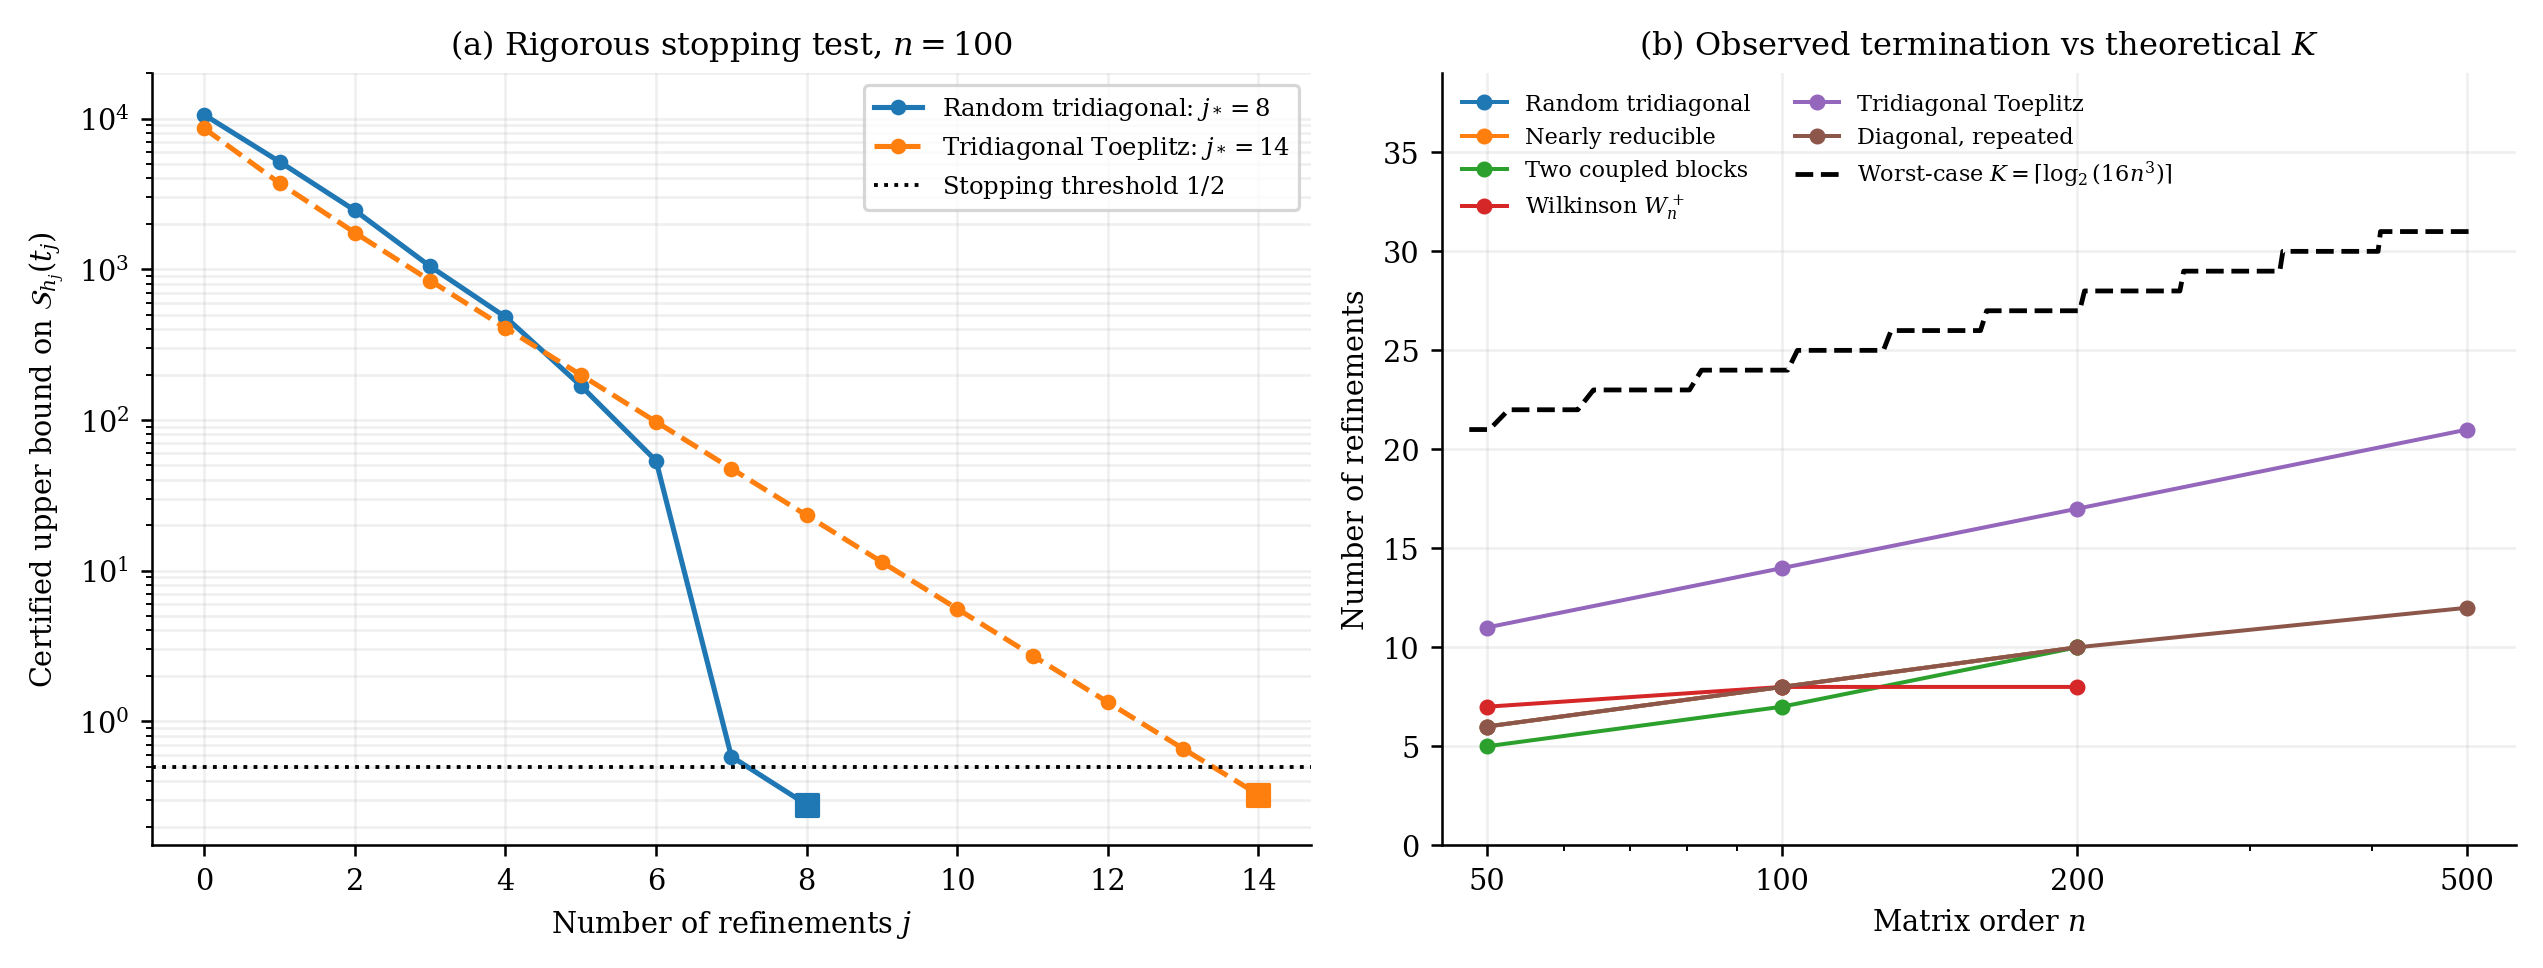
\includegraphics[width=\linewidth]{ke02_iterations_certified.png}
\caption{Certified stopping behavior. Left: rigorously enclosed
centered slope variation along representative selection paths at
$n=100$, with the stopping threshold $1/2$. Right: the observed
termination iteration $j_*$ compared with the theoretical upper
bound $K=\lceil\log_2(16n^3)\rceil$. The strict-Sturm
dataset includes all six families for $n=50,100,200$ and two
families for $n=500$.}
\label{fig:certified-iterations}
\end{figure}


\paragraph{Analytical versus directly certified spectral gaps.}
\label{subsec:numerical-certificates}

For the returned parameter and radius $(t_*,h_*)$, the local
certificate of \Cref{prop:bridge} gives
\begin{equation}\label{eq:numerical-slope-cert}
g_{\mathrm S}:=\frac{h_*^2}{2^{20}n^4}
<\gap(T+t_*X).
\end{equation}
Because the spectral oracle provides rigorous eigenvalue
enclosures
$\lambda_j(T+t_*X)\in[\underline\lambda_j,\overline\lambda_j]$,
we can also compute the independent lower bound
\begin{equation}\label{eq:numerical-direct-cert}
g_{\mathrm{dir}}
:=
\min_{1\leq j<n}
(\underline\lambda_{j+1}-\overline\lambda_j)
\leq\gap(T+t_*X).
\end{equation}
The second bound uses certified eigenvalue enclosures and is
not required by the interval-selection theorem.

\Cref{fig:certified-gaps} compares these two bounds with
the universal guarantee $2^{-34}\delta^2n^{-12}$.
The differences are substantial. For the random tridiagonal
matrix with $n=100$, we obtain approximately
\[
g_{\mathrm S}=5.98\times10^{-25},
\qquad
g_{\mathrm{dir}}=5.31\times10^{-4}.
\]
Thus the directly certified gap is more than twenty orders
of magnitude larger than the slope-based lower bound.

The experiments reveal two distinct sources of conservatism.
First, the worst-case iteration count is often unnecessary:
termination at $j_*<K$ retains a larger window and hence
a stronger slope-based certificate. Second, even at this
larger radius, the universal local certificate remains
much smaller than the actual certified gap. The second
effect is particularly pronounced for structured matrices,
including the Toeplitz family.

These observations identify the localization-to-gap
estimate of \Cref{sec:local-gap} as a natural target for further
theoretical improvement. They do not, by themselves,
imply a better worst-case exponent than $n^{-12}$.

\begin{figure}[h]
\centering
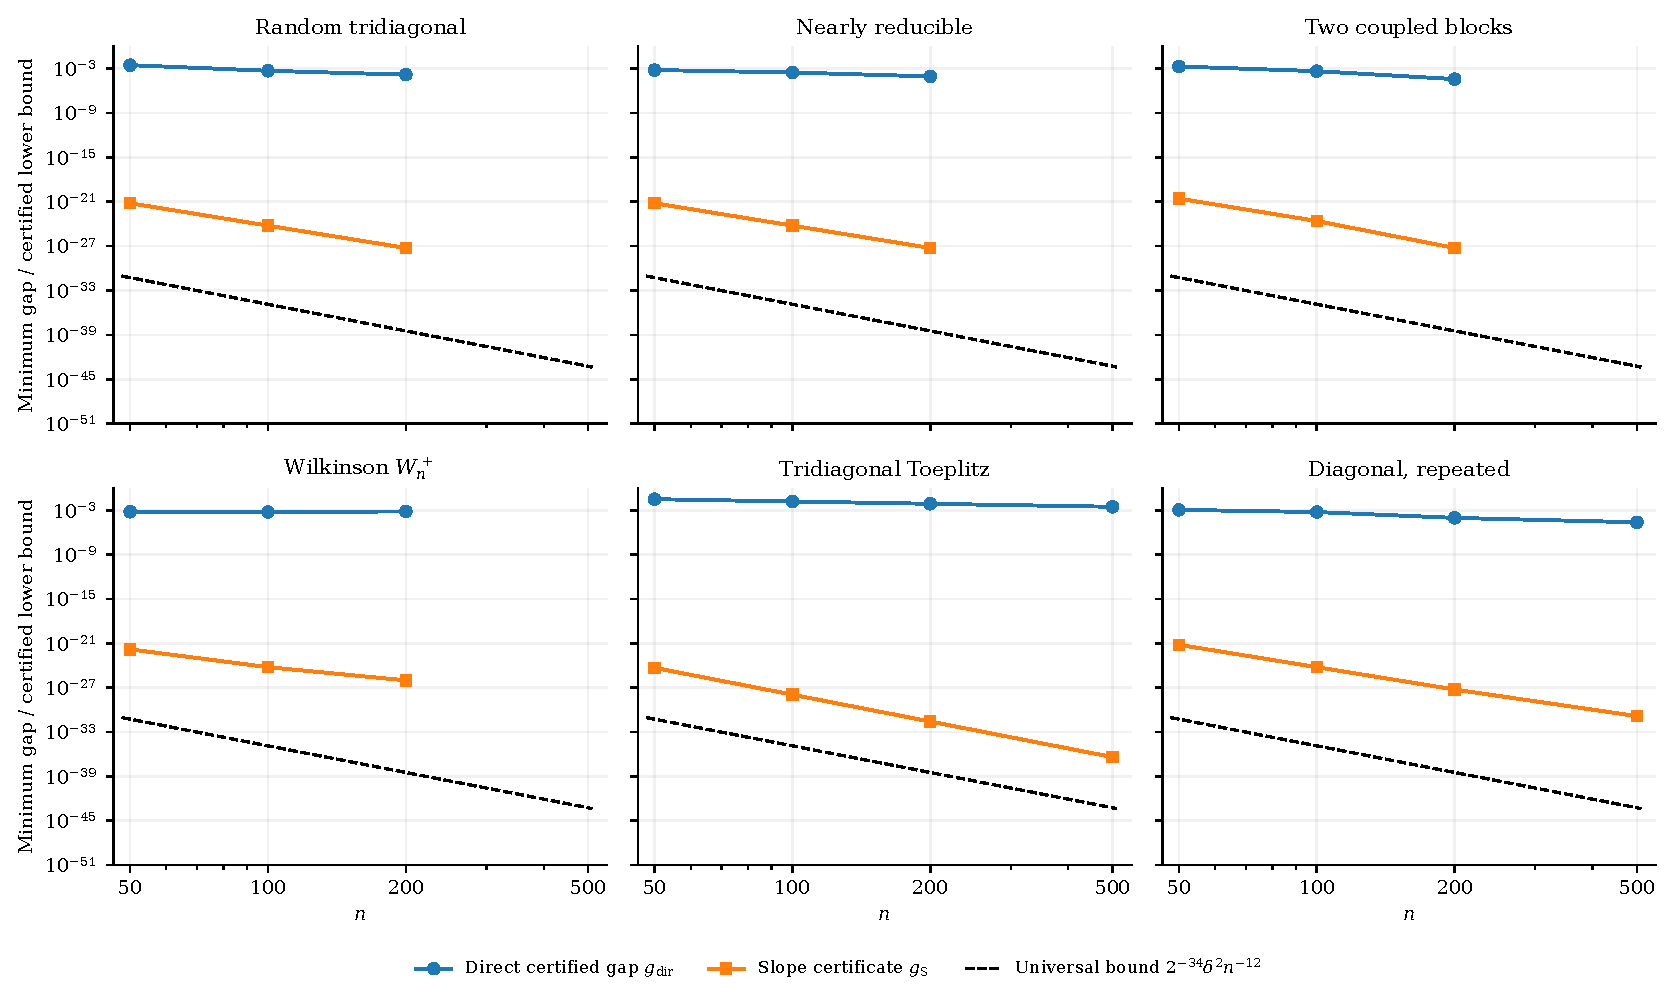
\includegraphics[width=\linewidth]{ke02_certified_gap_comparison.pdf}
\caption{Comparison of spectral-gap lower bounds for the six
test families. The solid curves give the directly certified
minimum gap; the square markers give the slope-based certificate
$g_{\mathrm S}$ at the actual stopping window. Dashed curves
show the universal lower bound
$2^{-34}\delta^2n^{-12}$. All displayed points use the
strict-Sturm dataset.}
\label{fig:certified-gaps}
\end{figure}


\paragraph{Finite-precision performance and scalability.}
\label{subsec:numerical-runtime}

The principal numerical difficulty is the evaluation of slope
differences over increasingly short windows. Subtraction of
nearby spectral-function values can substantially amplify
absolute evaluation errors. Consequently, double-precision
estimates of the stopping quantity can become unreliable at
moderate matrix orders.

The structured implementation avoids relying on a
double-precision error model for the final certificate.
Sturm bracketing supplies rigorous spectral enclosures,
and additional precision is requested only when the
current enclosure cannot decide the stopping condition.
A bisection fallback ensures that the refinement does
not depend solely on Newton convergence.

\Cref{fig:certified-runtime} reports the resulting runtime.
For the random matrix with $n=100$, the complete recorded
workflow takes approximately $0.93$ seconds. At $n=200$,
it takes about $4.0$ seconds. The Toeplitz family is
more demanding: its $n=200$ instance takes about
$17.7$ seconds, and the $n=500$ instance
takes approximately $238$ seconds.

These times include the preliminary double-precision
selection path and the subsequent rigorous certification.
They should not be interpreted as timings for a
nearly linear implementation of the theoretical oracle.

\begin{figure}[h]
\centering
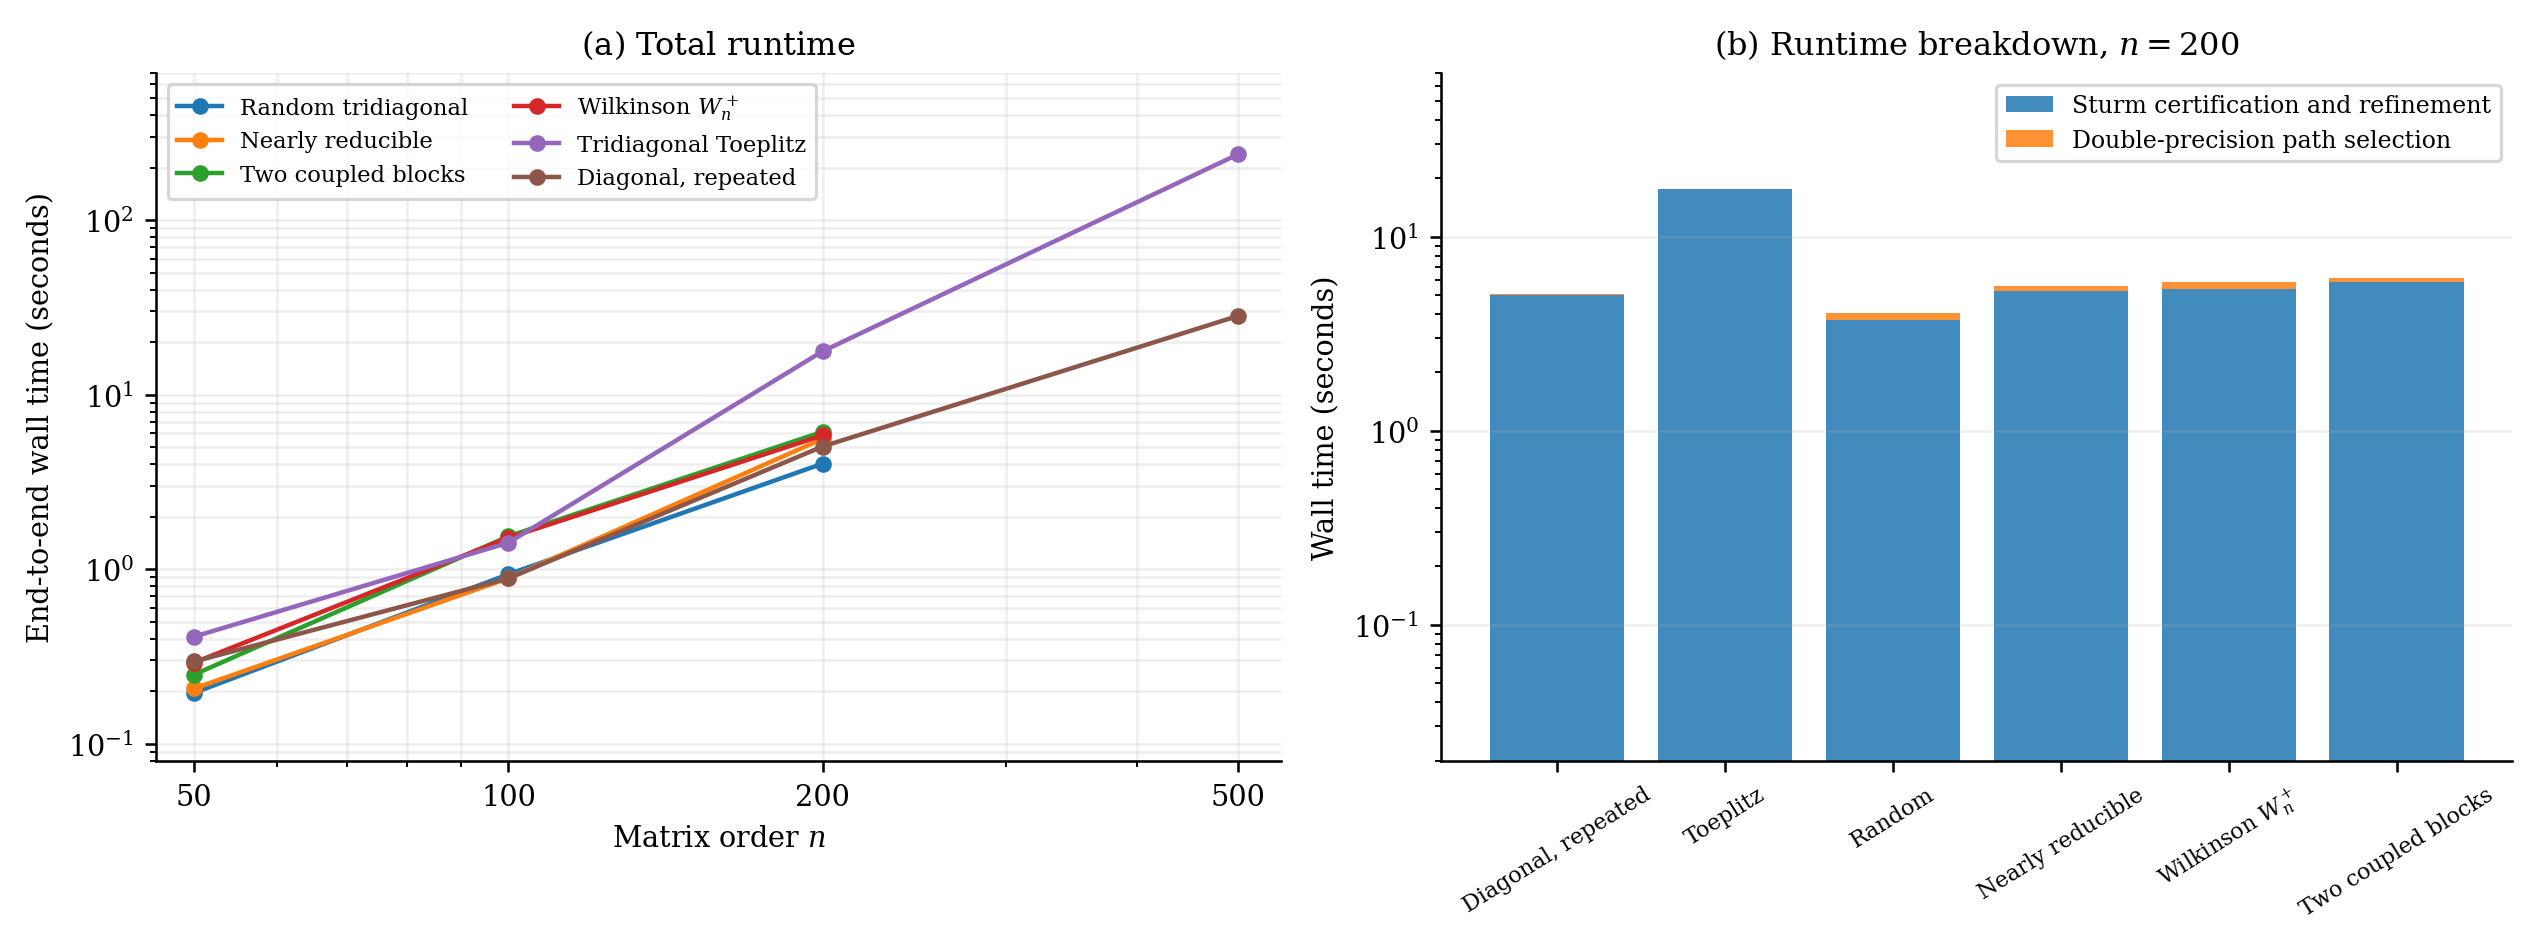
\includegraphics[width=\linewidth]{ke02_strict_runtime.png}
\caption{Runtime of the strict-Sturm implementation. Left:
total runtime across the reported matrix families and sizes.
Right: time spent on preliminary double-precision selection
and rigorous certification at $n=200$. The experiments
demonstrate the practical benefit of structure-exploiting
certification, without claiming the arithmetic complexity
of the oracle in \Cref{lem:oracle}.}
\label{fig:certified-runtime}
\end{figure}

\begin{table}[t]
\centering
\caption{Representative runs of the strict-Sturm implementation
with $\delta=0.48$. The index $j_*$ is the first refinement along
the uncertified double-precision selection path at which the
stopping test is rigorously certified. Runtime includes both selection
path construction and certification.}
\label{tab:certified-results}
\small
\begin{tabular}{lrrrrr}
\hline
Family and $n$ & $K$ & $j_*$ & $g_{\mathrm S}$
& $g_{\mathrm{dir}}$ & Time (s)\\
\hline
Random, 100       &24& 8&$5.98\times10^{-25}$&$5.31\times10^{-4}$&0.93\\
Toeplitz, 100     &24&14&$1.13\times10^{-28}$&$1.54\times10^{-2}$&1.42\\
Random, 200       &27&10&$5.63\times10^{-28}$&$1.58\times10^{-4}$&4.02\\
Wilkinson, 200    &27& 8&$9.71\times10^{-27}$&$6.97\times10^{-4}$&5.84\\
Toeplitz, 200     &27&17&$2.65\times10^{-32}$&$7.57\times10^{-3}$&17.72\\
Diagonal, 500     &31&12&$1.42\times10^{-31}$&$2.37\times10^{-5}$&28.25\\
Toeplitz, 500     &31&21&$4.04\times10^{-37}$&$2.99\times10^{-3}$&238.35\\
\hline
\end{tabular}
\end{table}

The results show that strict numerical certification with the
structured Sturm oracle is feasible at the orders reported in
\Cref{tab:certified-results}. The remaining bottleneck
is the cost of refining many eigenvalue enclosures, especially
for structured instances requiring more selection steps.


\paragraph{Comparison with alternative perturbations.}
\label{subsec:numerical-baselines}

We finally compare the deterministic selection rule with
several perturbations under the common budget $\|D\|_2\leq\delta$.
These include no perturbation, the fixed ramp $(\delta/n)X$,
a random parameter along the same direction, independent
random diagonal perturbations, and the best parameter on
a finite grid along the admissible segment.

\Cref{fig:certified-baselines} summarizes the comparison at
$n=100$. The paired baseline distributions come from a
double-precision sweep, while the overlaid strict
points give the directly certified gaps for representative
instances of the improved selector.

The deterministic selector is competitive with random
perturbations on the tested matrix families. In particular,
the structured Toeplitz examples illustrate that a suitable
diagonal direction can outperform unstructured diagonal
noise. The grid search can yield larger gaps, but it uses
many more trial parameters and does not supply the same
worst-case selection guarantee.

The purpose of our algorithm is not to maximize the minimum
gap along the admissible segment. Rather, it constructs a
parameter at which spectral separation can be certified
within a controlled number of refinements.

\begin{figure}[h]
\centering
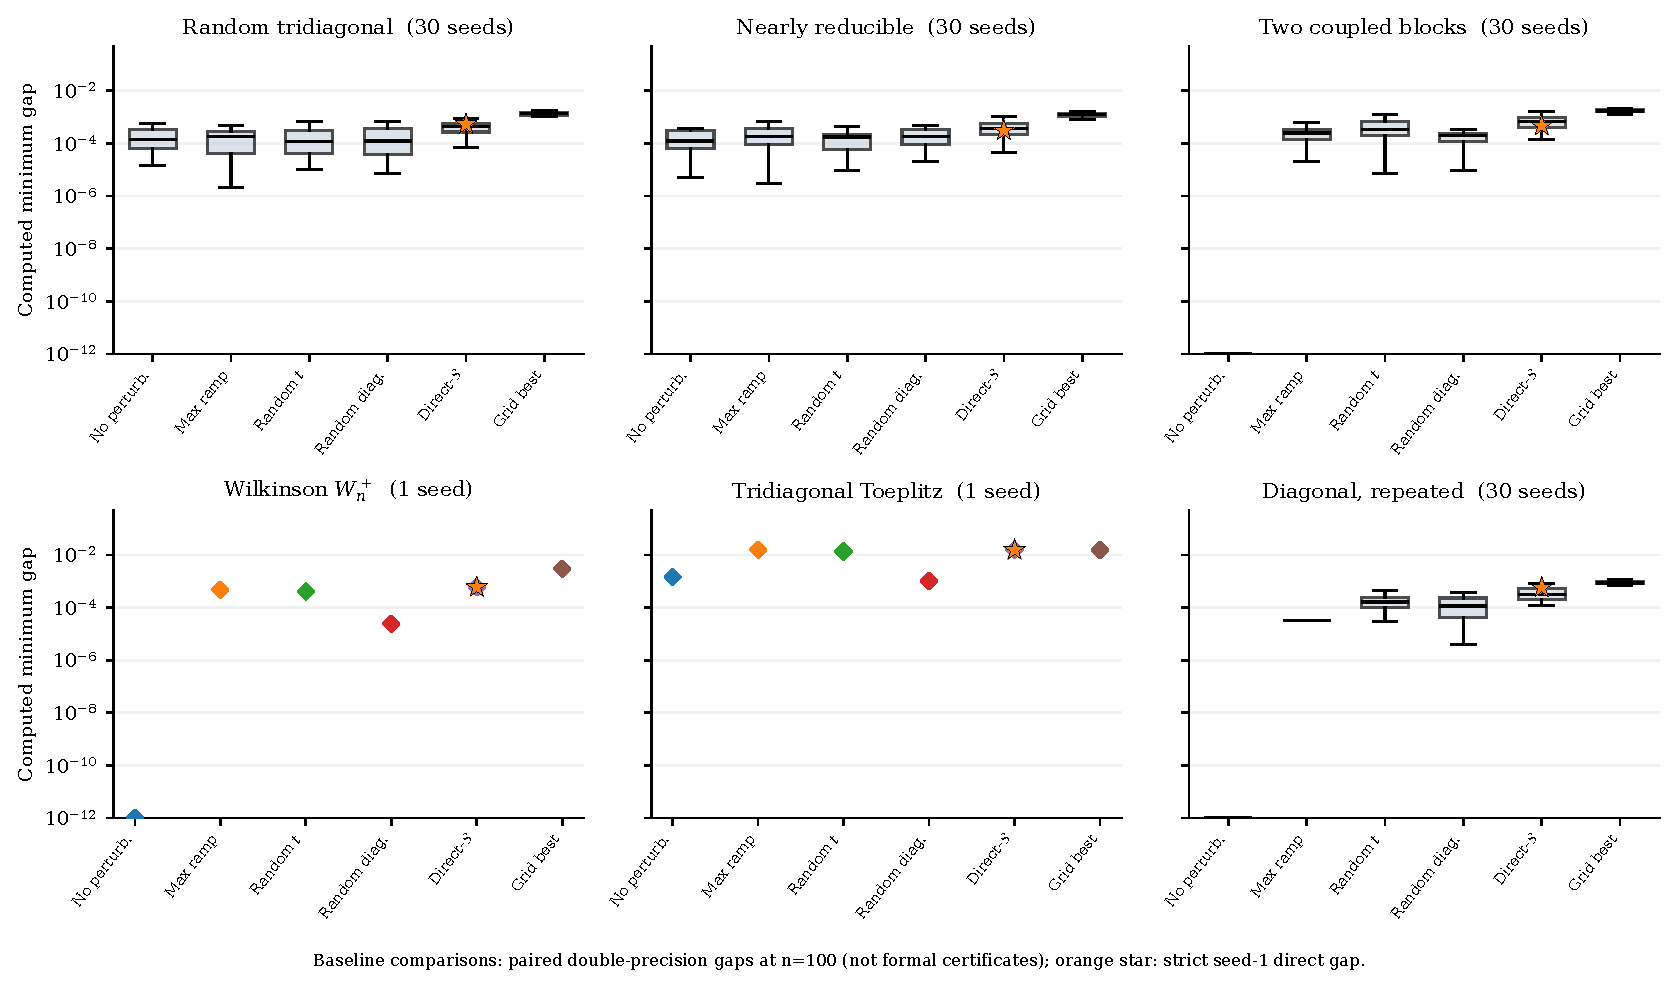
\includegraphics[width=\linewidth]{ke02_perturbation_baselines_new.pdf}
\caption{Comparison with alternative perturbations at $n=100$.
The paired distributions are computed in double precision
using a 30-seed baseline sweep. Orange stars
indicate the strict-Sturm direct gap for the representative
seed-1 output of the adaptive selector. The baseline
distributions are numerical comparisons, not formal
gap certificates.}
\label{fig:certified-baselines}
\end{figure}

For random
tridiagonal matrices and weakly coupled blocks, the selected
perturbation typically achieves a minimum gap two to three
times larger than the random baselines.

The advantage is particularly pronounced for structured
inputs. On the Wilkinson and Toeplitz examples, the selected
perturbation achieves substantially larger gaps than
independent random diagonal perturbations. For the Toeplitz
matrix, its performance is also close to the best parameter
found by grid search.

These comparisons illustrate the benefit of structured
perturbations and deterministic parameter selection.
The objective of our method, however, is not to maximize
the minimum gap, but to construct a perturbation with
a rigorous spectral-separation certificate and a
worst-case iteration guarantee.

\paragraph{Summary.}
The experiments support three conclusions. First, the
centered-slope stopping test often terminates well before
the theoretical limit $K$. Second, rigorous structure-aware
spectral computations make certified separation practical
at the reported dimensions, up to $n=500$. Third, the directly certified
gaps are typically many orders of magnitude larger than
the analytical lower bounds.

The main limitation of the theoretical gap guarantee thus
appears to lie in the conservatism of the universal local
certificate, rather than in the ability of the selector
to find a separating perturbation on these test matrices.
 

\section{Conclusions and outlook}
\label{sec:conclusion}

We have given a deterministic construction of a small diagonal
perturbation that produces inverse-polynomial spectral separation for
arbitrary Hermitian tridiagonal matrices. The proof combines
tridiagonal invariant-subspace localization with the variational geometry
of a convex weighted spectral function. Its finite-scale slope variation
provides a local gap certificate, while an adaptive, error-tolerant window
selector yields the global perturbation and a quantitative bound on the
number of refinements. With the exact-arithmetic spectral-function oracle of
\Cref{app:oracle}, the construction uses
$O(n[1+\log(n/\delta)]^3)$ arithmetic operations, comparisons and
square roots in total, and thus addresses the nearly linear
arithmetic version of the deterministic Minami perturbation problem.

The numerical illustrations, whose stopping tests are rigorously
certified, show that the stopping criterion often
succeeds well before the theoretical iteration bound. The structured
Sturm implementation also provides a practical means of certifying
individual eigenvalue enclosures and, consequently, lower bounds on the
actual minimum gap. These direct bounds are far larger than the
universal slope-based certificate on the tested matrices. Thus the
finite-scale selection mechanism performs well on these instances,
whereas the localization-to-gap constants and dimension dependence
remain natural targets for further analysis.

\paragraph{Sharper certificates and precision costs.}
The current local estimate combines an $O(n\sqrt\gamma)$
quasimode residual from the small-leakage cut with a stability
argument for a weighted spectral function. Understanding whether
classical localization techniques, including the complementary-block
analyses of Ye and Parlett and Nakatsukasa's blockwise sensitivity
bounds \cite{Ye1995,Parlett1996,VoemelParlett2011,Nakatsukasa2012},
can yield better dimensional dependence is an immediate question.
A second issue is finite-precision complexity. The nearly linear
arithmetic guarantee does not itself establish the cost in bits of
certified slope computations. An efficient bit-complexity analysis,
or a numerically better-conditioned finite-scale observable, would
further connect the theory to robust large-scale eigenvalue
preprocessing \cite{Sobczyk2025,GrafTownsend2026}.

\paragraph{Banded and block tridiagonal matrices.}
For bandwidth greater than one, the scalar three-term Wronskian
identity and the single-edge commutator are replaced by multi-component
boundary interactions. Moreover, the response of a multiple eigenspace
to the fixed diagonal ramp $X$ can be scalar even when the eigenspace
has dimension two. Thus a direct extension of the one-direction
local certificate is not automatic. The block tridiagonal perturbation
estimates of Nakatsukasa~\cite{Nakatsukasa2012} suggest studying
localization and response separation using several diagonal
directions, possibly with the number of directions depending on the
bandwidth rather than on $n$.

\paragraph{Multiple directions for general Hermitian matrices.}
For any two orthonormal vectors $u,v\in\mathbb C^n$, consider the
coordinate probes $E_i=e_ie_i^*$. Their compressions to
$\operatorname{span}\{u,v\}$ have eigenvalue spreads
$\Delta_i=|u_i|^2+|v_i|^2$, and hence
\[
\max_i\Delta_i\geq\frac2n.
\]
This shows that a predetermined family of $n$ coordinate directions
can distinguish the perturbation responses in every two-dimensional
subspace. Similarly, independent random sign diagonal probes satisfy
a mean-square response-separation estimate. These observations concern
\emph{detecting} a nearly degenerate eigenspace: they do not yet give
a single diagonal perturbation that simultaneously separates the
entire spectrum. Whether far fewer directions suffice for banded
matrices, or whether adaptive and randomized probes can be converted
into an efficient deterministic simultaneous-separation procedure,
remains an open direction of investigation. Related questions for
larger eigenspace clusters and complex Hermitian matrix families are
also natural, but require additional structure beyond the present
rank-two tridiagonal argument.

\paragraph{Beyond eigenvalue gaps.}
Diagonal separation may serve as a preprocessing component in
subspace iteration, deflation, and verified spectral computations,
including problems where eigenvectors and spectral projectors are
more sensitive than ordered Hermitian eigenvalues themselves.
The sketched subspace methods of Nakatsukasa and Tropp
\cite{NakatsukasaTropp2024} and the certified spectral approaches
of Colbrook and Townsend \cite{ColbrookTownsend2024,
ColbrookTownsend2025} provide useful, complementary algorithmic
contexts. Establishing an end-to-end improvement for a particular
parent eigensolver, rather than only a guaranteed separation bound,
is a further question.


\section*{Statements and Declarations}
\paragraph{Funding.}
The research of Wenqi Zhu was supported by the Engineering and Physical
Sciences Research Council under grant EP/Y028872/1, \emph{Mathematical
Foundations of Intelligence: An ``Erlangen Programme'' for AI}.

\paragraph{Competing interests.}
The authors have no competing interests to declare that are relevant to
the content of this article.

\paragraph{Data availability.}
The code and numerical experiments accompanying this paper, including
those of Section~\ref{sec:numerics}, are available at
\url{https://github.com/erenup/tridiagonal-spectral-separation}
(folder \texttt{verification/numerics/}).

\paragraph{Use of generative AI and AI-assisted technologies.}
During the preparation of this work, the authors used AI tools (Codex and Claude Code) to generate candidate constructions and code, perform computations, draft mathematical arguments, and improve the readability of the text. After using these
tools, the authors reviewed and edited the content as needed and take full
responsibility for the content of the publication. The theorems are
established by the written proofs; the numerical experiments in
Section~\ref{sec:numerics} are illustrations, in which rigorous
Sturm-based eigenvalue enclosures certify the stopping tests and the
directly certified gaps.

\appendix
\section{The spectral-function oracle: algebraic details}
\label{app:oracle}

We provide the arithmetic-model construction used in
\Cref{lem:oracle}. Let $A$ have diagonal entries $a_i$ and squared
off-diagonal magnitudes $c_i=|A_{i,i+1}|^2$. For complex
Hermitian $A$, each $c_i$ is computed as
$(\operatorname{Re}A_{i,i+1})^2+(\operatorname{Im}A_{i,i+1})^2$;
the off-diagonal entries enter only through the real numbers $c_i$,
so no phase gauge as in \Cref{rem:real} is computed. Since
$\norm A_2<2$, the numbers $r_j=2+\lambda_{n+1-j}(A)$ lie in $(0,4)$
and satisfy $r_1\geq\cdots\geq r_n$.
Form the monic polynomial
$P(z)=\det(zI+2I+A)=\prod_{j=1}^n(z+r_j)$.
Its tridiagonal determinant recurrence is
\[
P_0=1,\quad P_1=z+2+a_1,\qquad
P_i=(z+2+a_i)P_{i-1}-c_{i-1}P_{i-2}\quad(2\leq i\leq n).
\]
Writing this recurrence as a product of $2\times2$ polynomial
transfer matrices and multiplying with a balanced product tree
computes all coefficients of $P$ in $O(n[1+\log n]^2)$
exact arithmetic operations when degree-$m$ polynomial products
cost $O((m+1)[1+\log(m+1)])$. Such multiplication is available
through radix-two Fourier transforms. The required roots of unity
are constructed in the permitted arithmetic model from
nonnegative square roots by successive half-angle formulas.
Complex arithmetic in these transforms is carried out on pairs
of real numbers.

If $P(z)=E(z^2)+zO(z^2)$, apply the Graeffe transform
\[
G(P)(z)=E(-z)^2+zO(-z)^2=\prod_{j=1}^n(z+r_j^2).
\]
After $k$ iterations, $R=2^k$ and the transformed polynomial is
$\prod_j(z+r_j^R)$. Let $e_j$ be its positive elementary symmetric
coefficients, with $e_0=1$. Since $r_1\geq\cdots\geq r_n>0$, setting
$p_j=\prod_{i=1}^j r_i^R$ gives
$p_j\leq e_j\leq 2^n p_j$. Hence
\begin{equation}\label{eq:graeffe}
\boxed{r_j2^{-n/R}\leq
\left(\frac{e_j}{e_{j-1}}\right)^{1/R}
\leq r_j2^{n/R}.}
\end{equation}
Given $0<\eta<1$, let $k$ be the least integer with
$R\eta\geq8n$, where $R=2^k$. It is found by doubling $R$,
starting from $R=1$, and comparing $R\eta$ with $8n$; no
logarithm, floor or bit extraction is used as a primitive
operation, and $k=O(1+\log(n/\eta))$. Since $R\geq8n/\eta$, the approximation
$\widehat r_j=(e_j/e_{j-1})^{1/R}$ has
$|\widehat r_j-r_j|\leq4n/R\leq\eta/2$,
using $0<r_j<4$ and, for both sides of \eqref{eq:graeffe},
$1-2^{-x}\leq2^x-1\leq x$ for $0\leq x\leq1$, with $x=n/R$.
Taking the $R$th root requires $k$ successive nonnegative square
roots. The Graeffe iterations each
require polynomial squaring, giving
$O(n[1+\log n][1+\log(n/\eta)])$ arithmetic operations.

Set $\eta=\varepsilon/(\sum_{j=1}^n j)$ and
$\widehat\lambda_j=\widehat r_{n+1-j}-2$ for $1\leq j\leq n$.
The eigenvalues are matched index by index through
\eqref{eq:graeffe}: since $r_{n+1-j}=2+\lambda_j(A)$,
\[
|\widehat\lambda_j-\lambda_j(A)|
=|\widehat r_{n+1-j}-r_{n+1-j}|\leq\frac\eta2,
\qquad
\Bigl|\sum_jj\widehat\lambda_j-\sum_jj\lambda_j(A)\Bigr|
\leq\frac{n(n+1)}2\cdot\frac\eta2\leq\varepsilon.
\]
Since $\log(n/\eta)=O(1+\log(n/\varepsilon))$ and
$\log n<\log(n/\varepsilon)$, the combined arithmetic cost is bounded by
$O(n[1+\log(n/\varepsilon)]^2)$, as accounted for in the proof of
\Cref{lem:oracle}.
The Graeffe coefficients satisfy $e_j\leq2^n4^{nR}$, where
$R=\Theta(n^3/\varepsilon)$, and they can be exponentially large
in $nR$; for example, $e_n=2^{nR}$ when $A=0$. Their magnitudes
and bit lengths are not charged in the exact-arithmetic model,
so the oracle gives no bit-complexity bound.


\scriptsize{
\bibliographystyle{plain}
\bibliography{refs}
}
\end{document}
